\documentclass[journal]{IEEEtran}
\usepackage[T1]{fontenc}
\usepackage[utf8]{inputenc}
\usepackage{graphicx}
\usepackage{subcaption}
\usepackage{hyperref}
\pagestyle{plain}
\setlength{\parskip}{0.7em}  
\setlength{\parindent}{15pt}


\ifCLASSINFOpdf
  
\else
 
\fi





% correct bad hyphenation here
\hyphenation{op-tical net-works semi-conduc-tor}


\begin{document}
\title{Analysis of heart rate variability using mobile devices and machine learning}
\author{
    J. Bancerewicz, J. Kotłowski, O. Lozovyy, J. Morawska, M. Rzęsa\\
    \textit{Gdańsk University of Technology}\\
    \textit{Faculty of Electronics, Telecoummunications and Informatics}
}


% The paper headers
\markboth{}%
{Shell \MakeLowercase{\textit{et al.}}: Bare Demo of IEEEtran.cls for IEEE Journals}
\maketitle

\begin{abstract}
This paper presents methods of heart rate variability analysis based on electrocardiographic and photoplethysmographic signals obtained using mobile devices. An approach to processing the recorded data involving noise suppression, peak detection, and determining the intervals between impulses in the bodily processes was developed. Detection of R peaks in ECG and maxima of a PPG wave was performed using convolutional and recursive neural networks. The efficiency of the models was measured in comparison to the classic algorithms and reference data. The results show a high accuracy of peak identification and allow employing mobile devices to monitor cardiac parameters in both home environments and during physical activities.

% W niniejszej pracy przedstawiono metody analizy zmienności rytmu serca na podstawie sygnałów elektrokardiograficznych i fotopletyzmograficznych pozyskiwanych za pomocą urządzeń przenośnych. Opracowano proces przetwarzania zapisów obejmujący tłumienie zakłóceń, wykrywanie pików oraz wyznaczanie interwałów między impulsami w przebiegu fizjologicznym. Detekcję szczytów R w EKG oraz maksimów fali w PPG zrealizowano z wykorzystaniem splotowych i rekurencyjnych sieci neuronowych. Skuteczność modeli oceniono w odniesieniu do klasycznych algorytmów jak i danych referencyjnych. Wyniki wykazały wysoką dokładność identyfikacji pików oraz umożliwiają zastosowanie mobilnych systemów do monitorowania parametrów kardiologicznych w warunkach domowych i podczas aktywności fizycznej.

\textbf{Keywords---} heart rate variability; biomedical signals; electrocardiography; photoplethysmography; noise filtering; convolutional neural networks; peak detection; pulse-transit time; Pan-Tompkins algorithm; time analysis.
\end{abstract}
% zmienność rytmu serca; sygnały biomedyczne; elektrokardiografia; fotopletyzmografia; filtracja sygnałów; splotowe sieci neuronowe; detekcja szczytów; interwał propagacji tętna; algorytm Pan-Tompkins; analiza czasowa.

\section{Introduction}
% NOTE:(mati): czas rejestracji -> recording time? 
Heart rate variability is an important parameter in assessing cardiovascular health, as it reflects the balance between the sympathetic and parasympathetic nervous systems. Traditional HRV measurements conducted in clinical settings are characterized by high costs and limited recording durations. In recent years, advances in mobile technology have enabled the monitoring of cardiac activity in daily life.
% Zmienność rytmu serca stanowi istotny parametr oceny funkcjonowania układu sercowo-naczyniowego, odzwierciedlający równowagę pomiędzy aktywnością układu współczulnego i przywspółczulnego. Tradycyjne pomiary HRV prowadzone w warunkach klinicznych charakteryzują się wysokim kosztem oraz ograniczonym czasem rejestracji. W ostatnich latach postęp technologiczny w obszarze urządzeń przenośnych oraz sensorów optycznych umożliwił monitorowanie aktywności kardiologicznej w trakcie życia codziennego.

% NOTE:(mati): cel pracy -> purpose of the project?
\subsection{Aim of the study}
Beat detection techniques are applied to electrocardiographic (ECG) and photoplethysmographic (PPG) recordings and evaluated in terms of their usefulness for heart rate variability (HRV) analysis. Classical algorithms are compared with deep neural network–based approaches in terms of accuracy, robustness to noise, and applicability in real-world conditions. An Android mobile application records the PPG signal, while ECG data were acquired using a Polar H10 heart rate monitor. Both employ filtering, detection of characteristic points, and computation of HRV metrics. The quality of the signals obtained from mobile devices is validated against reference patterns. Heart rate parameters are compared with those derived from the electrocardiograph, and the precision of peak detection is assessed.
% Techniki detekcji uderzeń w zapisach elektrokardiograficznych i fotopletyzmograficznych są implementowane i oceniane względem użyteczności w analizie zmienności rytmu serca. Klasyczne algorytmy zestawia się z rozwiązaniami opartymi na głębokich sieciach neuronowych, uwzględniając skuteczność, odporność na zakłócenia oraz zastosowanie w warunkach rzeczywistych. Aplikacja mobilna rejestruje przebiegi PPG na platformie Android, dane EKG odczytuje się z pulsometru Polar H10, wykorzystując filtrację, identyfikację punktów charakterystycznych oraz wyznaczanie wskaźników HRV. Jakość sygnałów pozyskiwanych urządzeniami mobilnymi jest weryfikowana na podstawie wzorców referencyjnych, porównując parametry rytmu serca z elektrokardiogramu i określając precyzję wykrywania szczytów.

\newpage
% Techniki filtracji i modelowania sygnałów biomedycznych
\section{Filtration and biomedical signals modeling techniques}
Electrocardiography and photoplethysmography are among the most fundamental sources of biomedical signals used in modern diagnostic and monitoring systems. The signal processing is aimed at ensuring the reliability of physiological data in the presence of interference such as patient movements, environmental noise, and hardware limitations. Two dominant approaches are used: data filtering and artificial intelligence-based modeling. These approaches are often combined to improve the accuracy and robustness of the analysis in clinical settings \cite{1}.
% Elektrokardiografia i fotopletyzmografia należą do podstawowych źródeł sygnałów biomedycznych wykorzystywanych w nowoczesnych systemach diagnostycznych i monitorujących. Proces przetwarzania zapisów jest ukierunkowany na uzyskanie wiarygodnych informacji fizjologicznych przy obecności zakłóceń wynikających z ruchu pacjenta, interferencji środowiskowych i ograniczeń sprzętowych. Dominują dwa podejścia: filtrację danych oraz modelowanie wspierane sztuczną inteligencją, które są łączone  dla poprawy dokładności i zwiększenia odporności analizy w warunkach medycznych \cite{1}.

% Filtracja danych
\subsection{Data filtration}
Initial processing of physiological signals is based on interference elimination, improving the signal-to-noise ratio (SNR). Measurement errors caused by motion artifacts, power line interference at 50/60 Hz, and baseline wander are major sources of distortion in electrocardiography (ECG) and photoplethysmography (PPG) \cite{2}. Filtering enhances signal quality and improves the accuracy of feature detection as well as classification performance.
% Wstępne przetwarzanie przebiegów fizjologicznych opiera się na eliminacji zakłóceń, umożliwiając poprawę stosunku sygnału do szumu. W elektrokardiografii oraz fotopletyzmografii istotną rolę odgrywają niedokładności pomiarowe związane z ruchem, składowe sieciowe o częstotliwości 50/60 Hz oraz dryft linii izoelektrycznej \cite{2}. Filtracja podnosi jakość zapisu, poprawiając dokładność detekcji cech oraz efektywność klasyfikacji.

A band-pass filter restricting the frequency band to values characteristic of the given waveform is a fundamental method in signal analysis. The processing range is 0.5–40 Hz for ECG signals and 0.3–8 Hz for PPG signals, corresponding to the heart rate \cite{3}. Butterworth, Chebyshev, and elliptic filters, implemented in both IIR and FIR forms, are used in digital applications. FIR filters modeled using the window method provide stability and a linear phase response \cite{4}.
% Do podstawowych metod analizy sygnału należą filtry pasmowoprzepustowe, ograniczające pasmo częstotliwości do wartości charakterystycznych dla badanego przebiegu. Zakres przetwarzania zapisu EKG wynosi 0,5–40 Hz, natomiast PPG ogranicza się do 0,3–8 Hz, odpowiadającego rytmowi serca \cite{3}. W implementacjach cyfrowych wykorzystuje się filtry Butterwortha, Chebysheva, eliptyczne w postaci IIR oraz FIR projektowane metodą okienkową, zapewniające stabilność i liniową charakterystykę fazową \cite{4}. 

% NOTE:(mati): second sentence is a monster, i think i translated it well but it's a very complicated sentence
% NOTE:(mati): i translated eliminacja as cancellation based on the citation
Adaptive filters are applied to signals containing disturbances with varying parameters. LMS and RLS algorithms enable dynamic adaptation of system coefficients to signal characteristics, increasing the effectiveness of suppressing motion artifacts and power line interference. Notch filters are used to suppress the 50/60 Hz component \cite{5}.
% Dla sygnałów z zakłóceniami o zmiennych parametrach stosuje się filtry adaptacyjne. Algorytmy LMS i RLS umożliwiają dynamiczną adaptację współczynników układu do charakterystyki zapisu, zwiększając skuteczność tłumienia niestabilności ruchowych oraz interferencji sieciowych. W zastosowaniach medycznych mechanizmy notch zapewniają eliminację składowej 50/60 Hz \cite{5}.

\newpage
% TODO:(mati): eliminacja artefaktów impulsowych i krótkotrwałych?
% TODO:(mati): metody morfologiczne -> morphological methods?
Pulse artifacts and short-term impulse artifacts are suppressed using a median filter as well as morphological methods, which preserve diagnostic features such as QRS complexes \cite{6}. Empirical Mode Decomposition, Wavelet Packet Transform, and wavelet analysis enable signal decomposition into frequency components and selective noise suppression while preserving the structure of measurement peaks \cite{7}.
% Eliminacja artefaktów impulsowych i krótkotrwałych jest realizowana w oparciu o filtry medianowe oraz metody morfologiczne, umożliwiające zachowanie cech diagnostycznych, takich jak załamki QRS \cite{6}. Analiza falkowa oraz techniki Empirical Mode Decomposition i Wavelet Packet Transform zapewniają dekompozycję sygnału na składowe częstotliwościowe oraz selektywne tłumienie szumów przy utrzymaniu struktury pików przebiegu \cite{7}.

In advanced biomedical devices, algorithms based on probabilistic models are used. One such method is the Kalman filter, which estimates the actual measurement based on noise-affected observations \cite{8}. Another method is Independent Component Analysis, employed to separate signal sources and eliminate motion artifacts in photoplethysmography \cite{9}. Modern data isolation techniques combine traditional computing with machine learning. Signal refinement precedes feature extraction with neural networks, which increases the robustness of analysis under real-world conditions \cite{10}.
% W zaawansowanych zastosowaniach biomedycznych wykorzystuje się algorytmy oparte na modelach probabilistycznych. Jedną z metod jest filtr Kalmana, służący do estymacji rzeczywistego przebiegu na podstawie obserwacji obarczonych zakłóceniami \cite{8}, oraz Independent Component Analysis, stosowaną do separacji źródeł zapisu i eliminacji zniekształceń ruchowych w fotopletyzmografii \cite{9}. Współczesne techniki wyodrębniania danych integrują tradycyjne przetwarzanie z uczeniem maszynowym. Proces oczyszczania sygnału jest etapem poprzedzającym ekstrakcję cech z użyciem sieci neuronowych, zwiększając odporność analizy w warunkach naturalnych \cite{10}.

\subsection{Machine learning}
Artificial intelligence-based techniques represent one of the key approaches in biomedical signal analysis. The application of such algorithms enables automatic information extraction, reduces the reliance on preprocessing, and improves classification performance in the presence of interference. The literature emphasizes three primary solution categories.
% Techniki oparte na sztucznej inteligencji należą do kluczowych metod analizy sygnałów biomedycznych. Zastosowanie algorytmów umożliwia automatyczne wyodrębnianie informacji, ogranicza wpływ wstępnego przetwarzania i zwiększa skuteczność klasyfikacji w obecności zniekształceń. W literaturze wyróżnia się trzy główne rozwiązania.

Supervised approaches, including Support Vector Machines (SVM), k-Nearest Neighbors (k-NN), and Random Forests, are commonly used for heart rate measurement and arrhythmia detection. Logistic regression and linear discriminant analysis (LDA) provide simple and effective identification of signal patterns. The implementation of these methods in mobile diagnostic systems and monitoring devices, as well as their real-time processing, is enabled by the low computational complexity of the aforementioned techniques \cite{11}.
%Nadzorowane podejścia, obejmujące Support Vector Machines, k-Nearest Neighbors oraz Random Forest, są wykorzystywane do oceny rytmu serca oraz detekcji arytmii. Regresja logistyczna i liniowe modele dyskryminacyjne zapewniają prostą i efektywną identyfikację wzorców sygnałów.
%Niska złożoność obliczeniowa tych rozwiązań sprzyja implementacji w przenośnych systemach diagnostycznych i urządzeniach monitorujących, wspierając przetwarzanie danych w czasie rzeczywistym \cite{11}.

The second area focuses on sequential models, which capture temporal dependencies in electrocardiographic (ECG) and photoplethysmographic (PPG) signals. Recurrent neural networks (RNNs) and their extended forms, including Long Short-Term Memory (LSTM) networks and Gated Recurrent Units (GRUs), capture both short-term and long-term variations in the signal \cite{12}. Probabilistic models, such as Hidden Markov Models (HMMs), are alternatively used to identify anomalies and improve the effectiveness of dynamic heart rate analysis as well as the detection of cardiological abnormalities \cite{13}.
% Drugi obszar koncentruje się na modelach sekwencyjnych, umożliwiających odwzorowanie zależności czasowych w zapisach elektrokardiograficznych oraz fotopletyzmograficznych.
% Rekurencyjne sieci neuronowe i ich rozszerzone formy, w tym długa krótkoterminowa pamięć LSTM oraz jednostki z bramkowaniem pamięci GRU, rejestrują zarówno krótkotrwałe, jak i długookresowe zmiany sygnału \cite{12}. Alternatywnie są stosowane techniki probabilistyczne, w szczególności ukryte modele Markowa HMM, wspierające identyfikację anomalii oraz poprawiające skuteczność analizy dynamiki rytmu serca i detekcji nieprawidłowości kardiologicznych \cite{13}.

\newpage
% TODO:(mati): mehcanizm uwagi -> attention mechanism?
A commonly used approach is deep learning architectures, including convolutional neural networks (CNNs), which extract local features such as peak detection in PPG signals and QRS complexes in ECG signals \cite{14}. Transformer models based on the attention mechanism provide parallel mapping of temporal dependencies at multiple scales, increasing the system's robustness against motion artifacts and amplitude variability \cite{15}. Hybrid solutions, in which convolutional layers are combined with recurrent layers to integrate both local and global features within a single system, are gaining increasing relevance.
% Do najczęściej wykorzystywanych rozwiązań zalicza się architektury głębokiego uczenia, w tym konwolucyjne sieci neuronowe, przeznaczone do ekstrakcji cech lokalnych, takich jak detekcja szczytów w przebiegu PPG oraz zespołów QRS w sygnale EKG \cite{14}. Transformer, oparty na mechanizmie uwagi, zapewnia równoległe odwzorowanie zależności czasowych w wielu skalach, zwiększając odporność systemów na zakłócenia ruchowe i zmienność amplitudy \cite{15}. Rosnące znaczenie zyskują rozwiązania hybrydowe, w których warstwy splotowe są łączone z rekurencyjnymi, integrujące analizę lokalną i globalną w jednym układzie.


High resistance to interference and the ability to adapt to new datasets are characteristic features of machine learning. The transfer of models trained on large reference datasets to real-world clinical conditions is achieved through transfer learning, improving both generalization and classification accuracy \cite{16}.
%Uczenie maszynowe charakteryzuje się wysoką odpornością na zniekształcenia oraz adaptację do nowych zbiorów danych. Stosowanie podejścia transferowego realizuje przekształcenie modeli wytrenowanych na dużych bazach referencyjnych, do rzeczywistych warunków klinicznych, poprawiając generalizację oraz precyzję klasyfikacji \cite{16}.

% Ocena zmienności rytmu serca na podstawie przebiegów EKG i PPG
% TODO:(mati): second sentence is hell; is the translation accurate?
\subsection{Heart rate variability assessment based on ECG and PPG waveforms}
Photoplethysmographic signals are commonly used to estimate heart rate, while electrocardiography serves as the reference standard. The literature features both multichannel PPG datasets with parallel ECG recordings and ultra-short-term HRV analyses performed using deep learning algorithms.
%Sygnały fotopletyzmograficzne są powszechnie stosowane do estymacji tętna, natomiast elektrokardiografia pełni rolę standardu referencyjnego. W literaturze wyróżnia się badania poświęcone ultra-krótkoterminowej analizie HRV z wykorzystaniem głębokiego uczenia oraz prace udostępniające obszerne, wielokanałowe zbiory danych PPG z równoległym zapisem EKG.

% TODO:(mati): odwzorować is not recreate but no better idea
% TODO:(mati): last sentence is complicated, double check
End-to-end approach to evaluating heart rate variability parameters from 10-second fragments of optical measurements was developed in the Wang i Najafizadeh paper \cite{17}. To recreate the necessary features a recursive LSTM neural network was employed. Cardiographic reference signal was registered using a standard clinical system. Acquired coefficients of correlation to reference values exceeded 0.9 with average relative error below 10\% which signifies a high accuracy of the model for any minimal-length sample.
%Podejście end-to-end do szacowania parametrów zmienności rytmu serca z 10-sekundowych fragmentów przebiegu optycznego opracowano w pracy Wang i Najafizadeh \cite{17}. Do odwzorowania niezbędnych cech zastosowano rekurencyjną sieć neuronową LSTM. Sygnał odniesienia kardiograficzny rejestrowano przy użyciu standardowego systemu klinicznego, a uzyskane współczynniki korelacji z wartościami wzorcowymi przekraczały 0,9, z średnim błędzie względnym poniżej 10\%, wskazując dokładność modelu dla minimalnej długości próbki.

The UTSA-PPG dataset \cite{18} was published in 2025. It contains hours-long recordings of photoplethysmographic (PPG) signals with parallel electrocardiographic (ECG) measurements, supplemented with accelerometer data. Heart rate analysis showed an average deviation of less than 2 beats per minute, and the correlation with ECG for basic HRV indicators ranged from 0.85 to 0.95, depending on the metric used. Machine learning techniques, including decision trees and multilayer perceptrons, were employed for signal processing, enabling precise profile reconstruction. Integrating these models into a hybrid approach improved accuracy and reduced error. The variety of samples supports the development of architectures capable of high generalization.
% Zbiór UTSA-PPG \cite{18} został opublikowany w 2025 roku, obejmujący wielogodzinne rejestracje zapisów fotopletyzmograficznych oraz równoczesny przebieg elektrokardiograficzny, uzupełniony o dane z akcelerometru. Analiza HR odnotowała średnią wartość odchylenia poniżej 2 uderzeń na minutę, a dla podstawowych wskaźników HRV stopień powiązania z EKG wynosił 0,85-0,95 w zależności od przyjętej metryki. Do przetwarzania sygnałów wprowadzono techniki uczenia maszynowego, jak drzewa decyzyjne i wielowarstwowe perceptrony, umożliwiające dokładne odwzorowanie charakterystyk. Integracja tych modeli w metodzie hybrydowej przyczyniła się obniżenia błędu oraz poprawy precyzji uzyskanych wyników. Zróżnicowanie próbek sprzyja opracowaniu architektury o wysokiej zdolności do generalizacji.

% TODO:(mati): obrazowanie w trybie kontaktowym?
% TODO:(mati): poziom zgodności?
\newpage
De Ridder et al. \cite{19} conducted a systematic review of mobile applications based on optical pulse measurements, which acquire data in contact mode with a sampling frequency determined by the frame rate. Validation studies in controlled environments confirmed strong agreement between heart rate values and cardiac signals, with consistency levels ranging from 0.95 to 0.99 and an absolute error below 2 beats per minute \cite{20}. A lower fit was observed for short deviation intervals, with correlation values of 0.75–0.85. Results deteriorated further in everyday environments due to motion artifacts, necessitating the use of filtering and data correction procedures to handle distorted signals.
%De Ridder i in. \cite{19} przeprowadzili przegląd systematyczny aplikacji mobilnych bazujących na optycznej procedurze pomiaru pulsu, pozyskując przebieg poprzez obrazowanie w trybie kontaktowym, z częstotliwością próbkowania zależną od liczby klatek na sekundę. Badania walidacyjne w warunkach kontrolowanych potwierdziły zbieżność wartości tętna z sygnałem sercowym o poziomie zgodności w zakresie 0,95–0,99 oraz błędzie absolutnym poniżej 2 uderzeń na minutę \cite{20}. Dla prostych odchyleń interwałów zaobserwowano niższe dopasowanie, z korelacją rzędu 0,75–0,85. W środowisku codziennego użytkowania wyniki ulegają pogorszeniu wskutek zakłóceń ruchowych, wymagając zastosowania filtracji oraz procedur eliminacji zniekształconych danych.


%Opis systemu i danych
%Akwizycja danych
%Akwizycja danych EKG
\section{System and data characterization}
\subsection{Data acquisition}
\subsubsection{ECG data acquisition}
Data used for R-peak detection model training and validation was acquired using the Polar H10 heart monitor, which is capable of recording electrocardiographic signals at a sampling frequency of 130 Hz. This resolution enables the creation of a profile essential for HRV analysis.
% Dane wykorzystane do trenowania i walidacji modelu detekcji załamków R zostały pozyskane za pomocą pulsometru Polar H10, zdolnego do rejestrowania sygnału elektrokardiograficznego z częstotliwością próbkowania wynoszącą 130 Hz. Przyjęta wartość umożliwia charakterystykę przebiegu istotną dla analizy HRV.

The Polar H10 sensor is a heart rate detector commonly used in sports and diagnostics. The device employs chest electrodes to register electric potentials associated with cardiac activity, providing higher measurement precision compared to optical methods. Data transmission is carried out via the Bluetooth Low Energy (BLE) standard, while internal memory allows offline storage of recordings. The accuracy of the Polar H10 is comparable to that of single-channel ECG systems used in clinical diagnostics, making mobile signal acquisition feasible \cite{21}.
%Sensor Polar H10 jest czujnikiem tętna stosowanym w sporcie oraz diagnostyce. Działanie urządzenia opiera się na elektrodach piersiowych rejestrujących potencjały elektryczne związane z aktywnością serca, zapewniając wyższą precyzję pomiaru w porównaniu z metodami optycznymi. Transmisja przebiegu realizowana jest poprzez standard Bluetooth Low Energy, a pamięć wewnętrzna umożliwia zapis danych w trybie offline. Dokładność detekcji Polar H10 jest zbliżona do systemów EKG jednokanałowych stosowanych w diagnostyce klinicznej, umożliwiając zastosowanie w mobilnym rejestrowaniu sygnału \cite{21}.

Two-hour measurement sessions were conducted with five participants to collect the required amount of data. The recorded signals varied in terms of physical activity level, heart rate variability, and the presence of sudden body movements causing measurement artifacts. Data was transmitted in real time in 13-point packets, consistent with the established sampling rate, and subsequently stored in CSV format.
%W celu zgromadzenia odpowiedniego zbioru danych przeprowadzono dwugodzinne eksperymenty pomiarowe z udziałem pięciu osób. Rejestrowane zapisy były zróżnicowane pod względem poziomu aktywności fizycznej, zmienności rytmu serca, a także obecnością nagłych ruchów ciała, prowadzących do zakłóceń przebiegu. Sygnał przesyłano w czasie rzeczywistym w pakietach po 13 punktów zgodnych z przyjętą częstotliwością próbkowania i zapisywano w formacie CSV. 


% Akwizycja danych PPG
% Aplikacja mobilna
\subsubsection{PPG data acquisition}
\paragraph{Mobile application}
An Android-based application utilizing the photoplethysmographic method for heart rate measurement was developed. Signal acquisition was performed by placing the participant’s fingertip directly on the camera lens, illuminated by the integrated LED light source. This setup enabled the detection of optical changes caused by cyclical variations in blood volume within the skin’s microvascular vessels.
%Zaprojektowano oprogramowanie w systemie Android realizujące pomiar tętna metodą fotopletyzmografii. Rejestrację sygnału przeprowadzono poprzez umieszczenie opuszka palca bezpośrednio na obiektywie kamery oraz zintegrowanym źródle LED, umożliwiając detekcję zmian optycznych wywołanych cyklicznymi wahaniami objętości krwi w tkankach skórnych. 
\newpage
Heart rate monitors are widely applied in clinical environments to acquire photoplethysmographic measurements, where they are characterized by high precision and stability. In mobile applications, the signal quality is generally sufficient for use in home environments, while maintaining the advantages of universality, low cost, and broad hardware accessibility.
% Dla zastosowań klinicznych wykorzystuje się pulsometry do pozyskiwania przebiegu PPG, cechujące się wysoką precyzją i stabilnością akwizycji. W środowisku mobilnym jakość odczytanego zapisu jest wystarczająca, zapewniając działanie w warunkach domowych przy zachowaniu uniwersalności pomiarów, niskiego kosztu i łatwej dostępności sprzętu.


\begin{figure}[htbp]
    \centering
    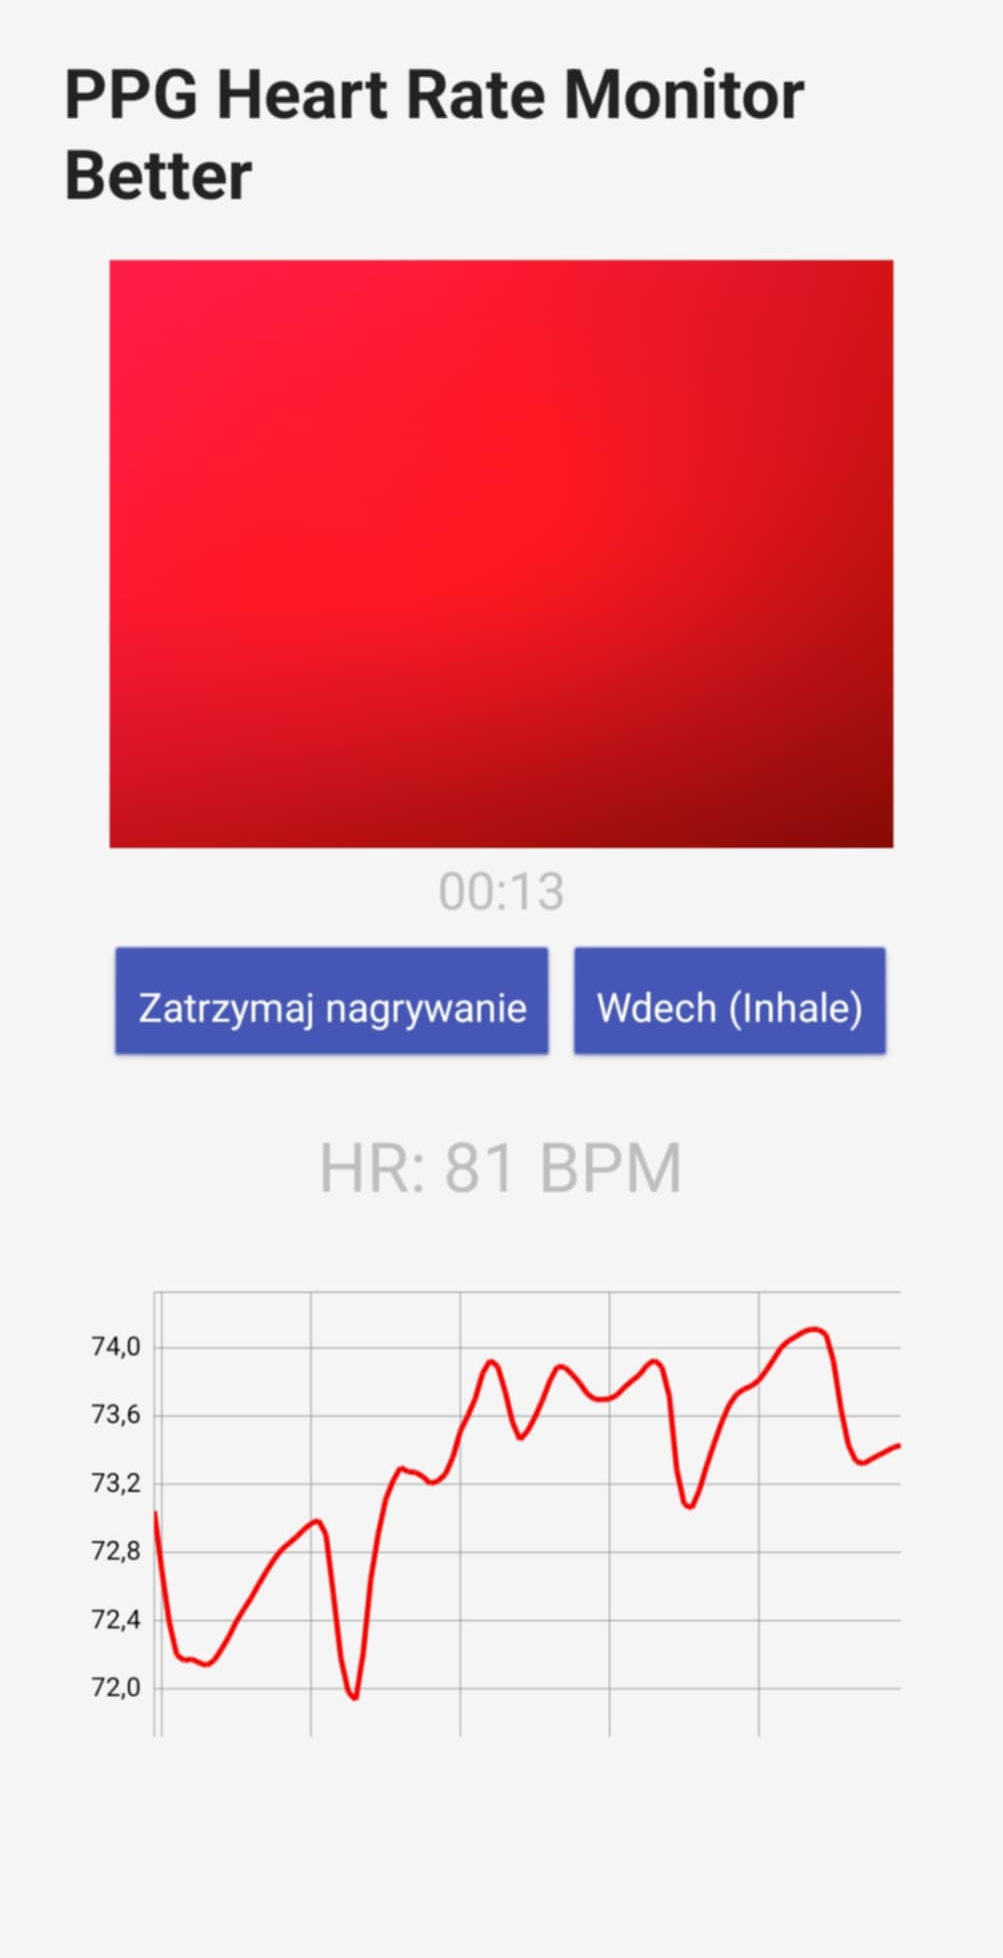
\includegraphics[scale=0.17]{aplikacja.png}
    \caption{Mobile app interface}
    \label{fig:aplikacja_mobilna}
\end{figure}


The application displays PPG waveforms in real time as a dynamically updating heart rate chart. Simultaneously, timestamps corresponding to inhale and exhale events are registered, enabling correlation with the PPG signal. This allows for analysis of the relationship between the respiratory cycle and its associated parameters.
%Aplikacja prezentuje przebieg PPG w czasie rzeczywistym w postaci dynamicznego wykresu zmian rytmu serca. Zarejestrowane znaczniki czasowe odpowiadające momentom wdechu i wydechu umożliwiają korelację z sygnałem w celu analizy zależności między cyklem oddechowym a jego parametrami.


The recorded signal is processed using a low-pass filter. Peak detection is performed by analyzing three consecutive samples of the signal, where the central point is classified as a peak if its value exceeds that of its neighboring points. To prevent false identifications caused by motion artifacts, a newly detected peak is only acknowledged if it occurs at least 600 ms after the previous one. Each identified extremum is stored together with its timestamp and subsequently used to dynamically calculate the Beats Per Minute (BPM) according to Equation (1):
%Zarejestrowany zapis ulega filtracji dolnoprzepustowej. Detekcja lokalnych maksimów realizowana jest poprzez analizę trzech kolejnych próbek sygnału, środkowy punkt klasyfikowany jest jako szczyt, jeśli jego wartość przewyższa oba sąsiednie. Akceptacja następnego piku wymagana upływu co najmniej 600 ms od poprzedniego wykrycia, ograniczając błędne rozpoznania wynikające z zakłóceń ruchowych. Zidentyfikowane ekstremum jest rejestrowane wraz ze znacznikiem czasu i wykorzystywane do dynamicznego wyznaczania częstości uderzeń serca BPM, zgodnie z równaniem (1) :

\begin{equation}
\text{BPM} = \frac{60}{\Delta t}
\label{eq:bpm}
\end{equation}
where $\Delta t$  - average time span between consecutive signal peaks

%Opracowana aplikacja mobilna została udostępniona publicznie pod adresem:
The source code of the developed mobile application has been hosted at the address:
\href{https://github.com/JanBancerewicz/PPGbetter}{https://github.com/JanBancerewicz/PPGbetter}

\newpage
%Proces rejestracji sygnału
\paragraph{Signal recording method}
Data used to train and validate the wave peak detection model was acquired using the developed application. Images were captured in real time in the YUV 4:2:0 format at a resolution of 640×480 pixels. From each frame, the luma component was extracted, and the average brightness value was computed. The resulting value represents a single sample of the raw photoplethysmographic signal.
%Dane wykorzystane do trenowania i walidacji modelu detekcji szczytów fali zostały pozyskane przy użyciu zaprojektowanej aplikacji. Obrazy przechwytywano w czasie rzeczywistym w formacie YUV 4:2:0 o rozdzielczości 640×480. Z każdej klatki wyodrębniano składową luminancji, na podstawie której obliczano średnią wartość jasności pikseli. Otrzymany odczyt stanowił pojedynczą próbkę surowego sygnału fotopletyzmograficznego.

A series of measurements involving six participants was conducted to collect the required amount of data. Each session lasted 10 minutes and included signal recording under varied conditions, with small finger movements also taken into account.
%W celu zgromadzenia odpowiedniego zbioru danych zrealizowano serię pomiarów z udziałem sześciu osób. Każda sesja trwała 10 minut i obejmowała rejestrację sygnału w zróżnicowanych warunkach, uwzględniających drobne ruchy palca wpływające na zmienność przepływu krwi.

Data transmission between the smartphone and the server was carried out using the WebSocket protocol. The data was sent in packets containing individual measurement points along with their corresponding timestamps. The sampling frequency was consistent with the frame rate, averaging about 30 Hz. The received data was buffered on the server and stored in CSV format.
% Transmisję danych pomiędzy smartfonem a komputerem przeprowadzono z wykorzystaniem protokołu WebSocket. Informacje przesyłano w pakietach zawierających pojedyncze punkty pomiarowe wraz z odpowiadającymi im znacznikami czasu. Częstotliwość próbkowania była zgodna z liczbą klatek wideo, wynoszącą około 30 Hz. Odebrane dane buforowano na komputerze i zapisywano w formacie CSV.

%Filtracja sygnału – filtr Butterwortha
% TODO:(mati): first sentence - double check
% TODO:(mati): monotoniczne tłumienie, zbocze przejściowe
\subsection{Signal filtration – Butterworth filter}
The Butterworth filter was originally developed as an analog solution with a maximally flat amplitude response in the passband, minimizing oscillations and signal distortions. It is characterized by monotonic attenuation in the stopband and a gentler transition slope compared to higher-selectivity structures such as Chebyshev and elliptic filters \cite{22}. In digital implementations, it is realized as an Infinite Impulse Response (IIR) system, where each output sample depends on both current input values and previous output values. This approach allows the deployment of higher-order filters with a limited number of coefficients, making it suitable for real-time applications \cite{23}.
%Filtr Butterwortha opracowano jako rozwiązanie analogowe o maksymalnie płaskiej charakterystyce amplitudowej w paśmie przepustowym, minimalizującej oscylacje i zniekształcenia sygnału. Charakteryzuje się monotonicznym tłumieniem w paśmie zaporowym oraz łagodniejszym zboczem przejściowym niż w strukturach o wyższej selektywności, w tym Czebyszewa i eliptycznych \cite{22}. W implementacji cyfrowej przyjmuje postać układu o nieskończonej odpowiedzi impulsowej IIR, gdzie bieżąca próbka wyjściowa zależy od wartości wejściowych, jak i poprzednich stanów wyjściowych. Podejście to umożliwia realizację filtrów wyższych rzędów przy ograniczonej liczbie współczynników, wykorzystywanych w aplikacjach czasu rzeczywistego \cite{23}.

\begin{figure}[htbp]
    \centering
    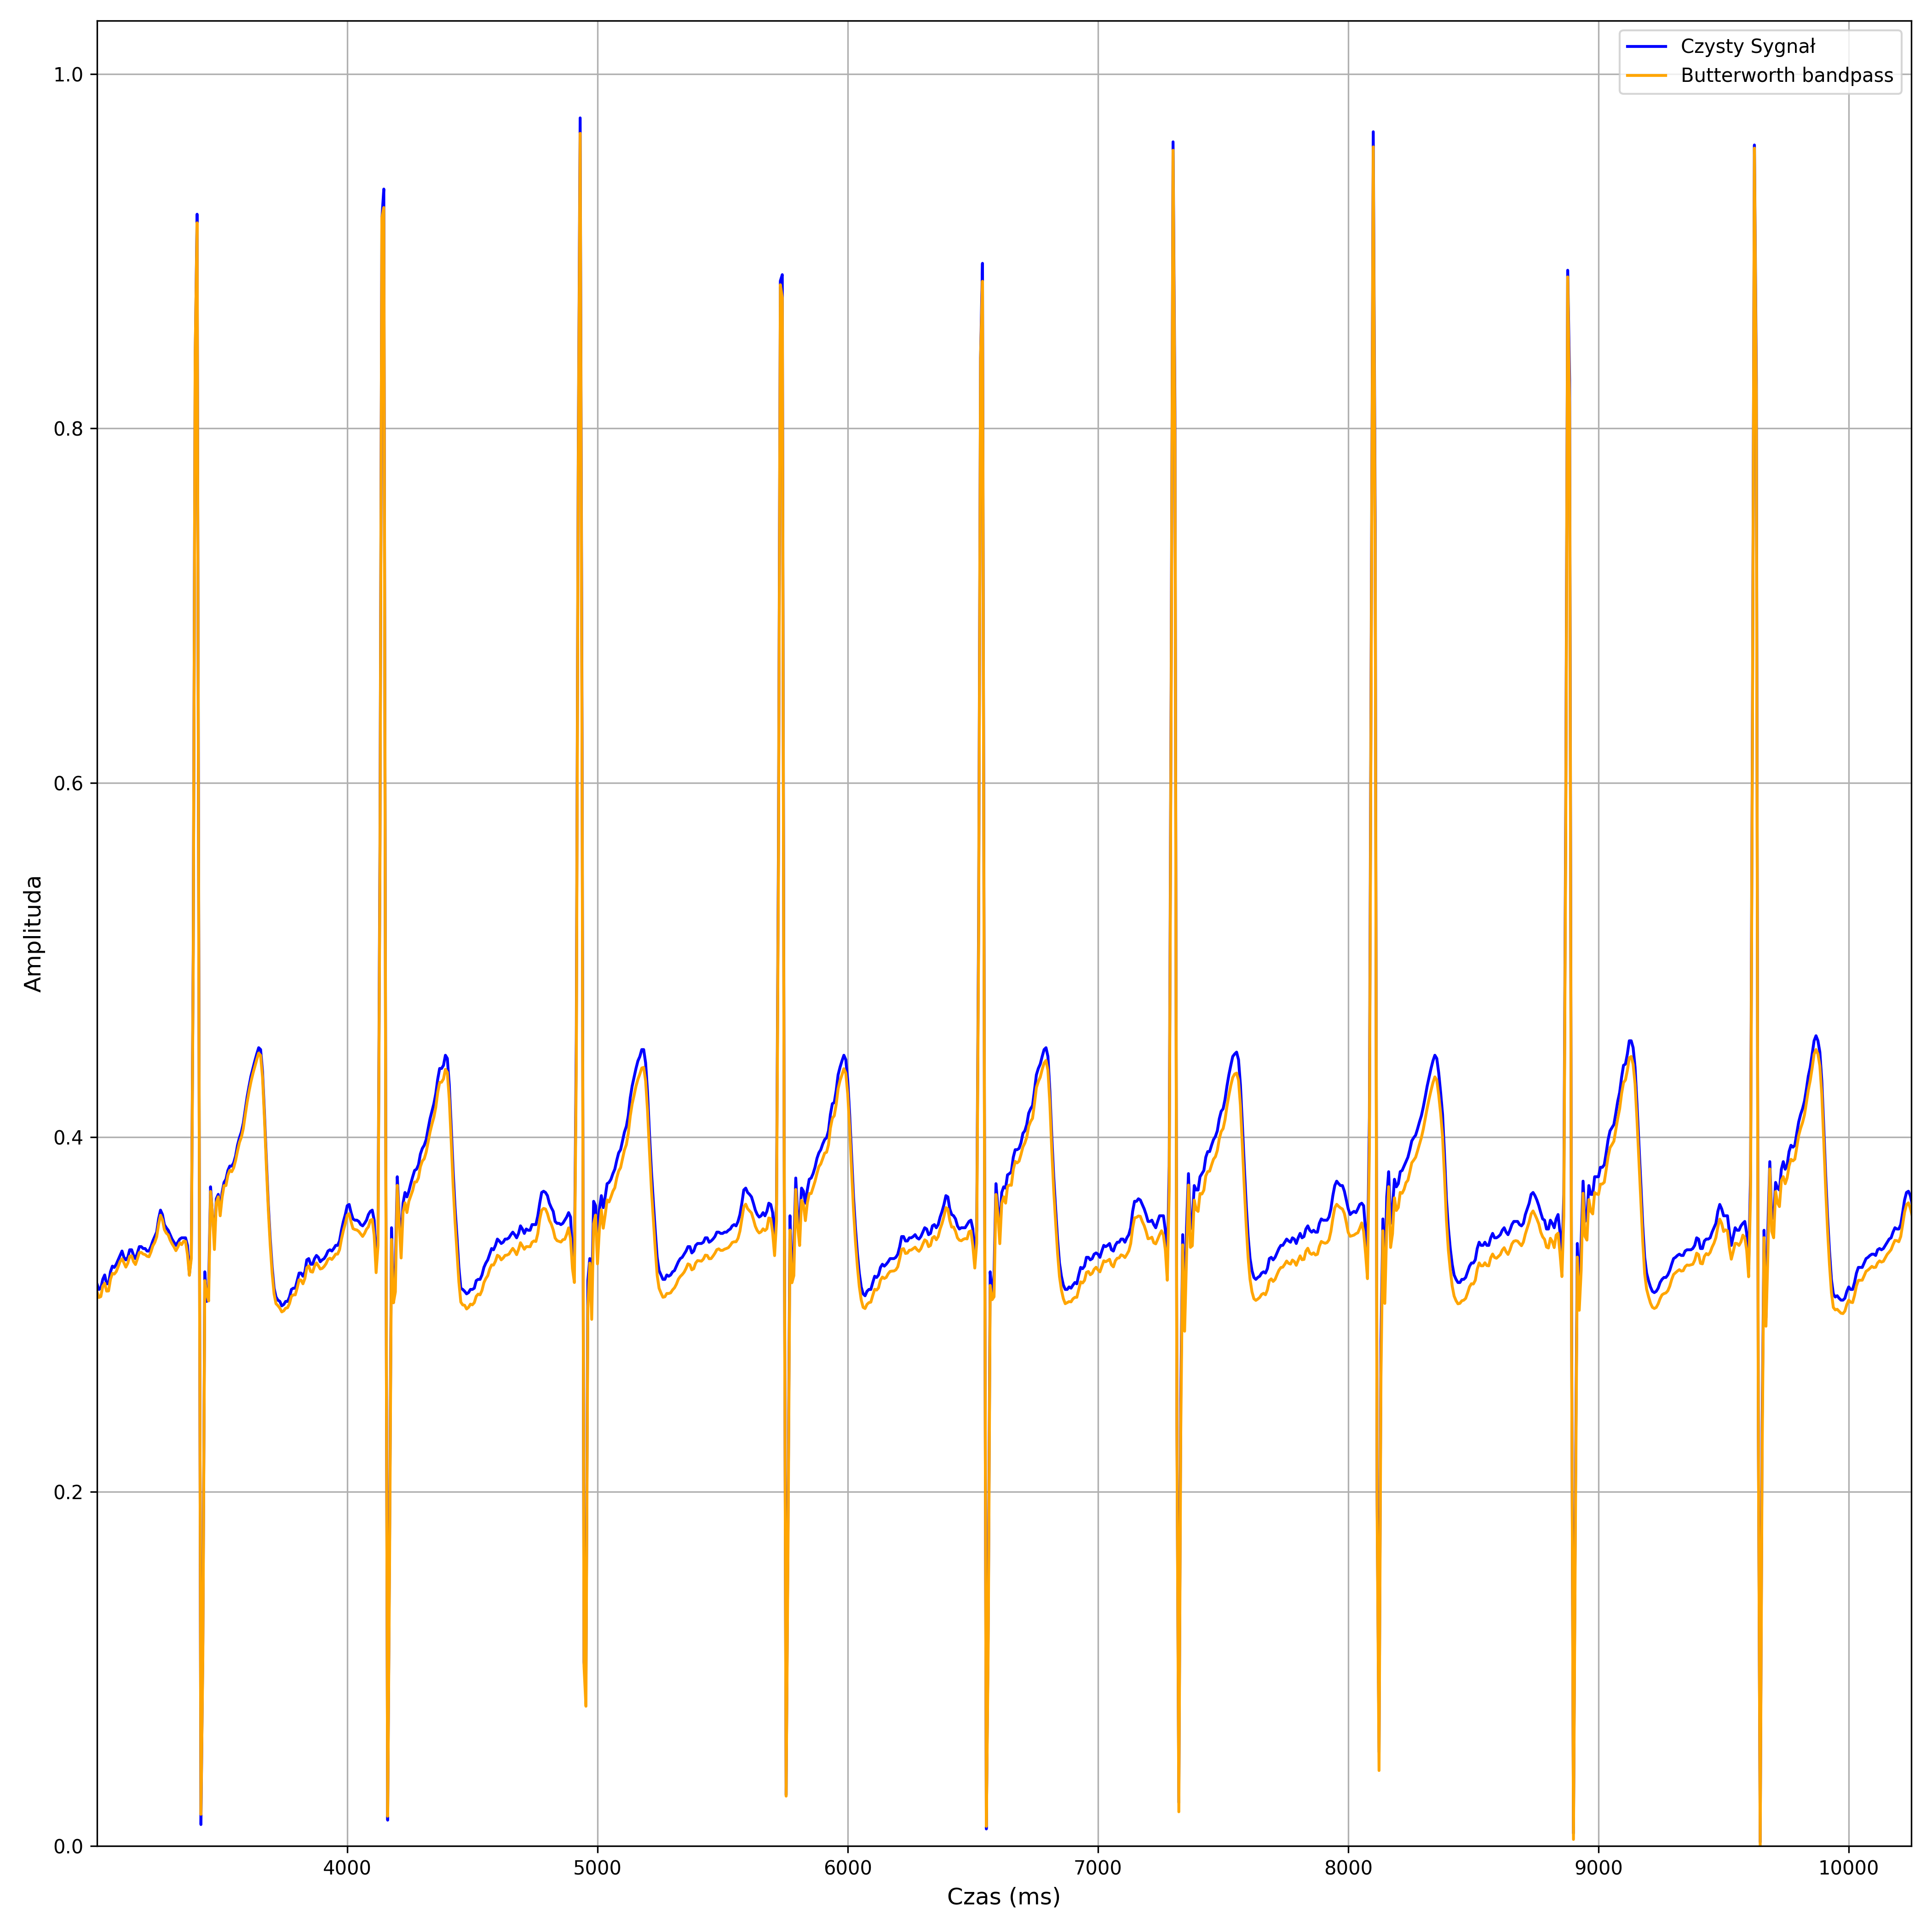
\includegraphics[width=0.76\linewidth]{Filtr_EKG.png} 
    \caption{A comparison between raw and filtered ECG signals}
    \label{fig:filtr_ekg}
\end{figure}

A fifth-order digital filter was employed to process the ECG signal. The filter has a passband frequency range of 0.5 Hz to 45 Hz and suppresses both noise and interference. The lower cutoff frequency reduces slow baseline variations caused by body movements or unstable electrode placement \cite{24}, while the upper cutoff frequency attenuates power line, electromagnetic, and muscle artifacts \cite{25}. Signal filtration was performed using the NeuroKit2 library.
%Do przetwarzania sygnału EKG wykorzystano cyfrowy filtr piątego rzędu o charakterystyce pasmowo-przepustowej, obejmującej zakres częstotliwości od 0,5 Hz do 45 Hz, eliminujący szumy oraz zakłócenia. Dolna granica pasma redukuje powolne zmiany w zapisie wywołane ruchem ciała lub niestabliną pozycją elektrod  \cite{24}. Natomiast górna tłumi zakłócenia sieciowe, elektromagnetyczne oraz mięśniowe  \cite{25}. Filtracja danych została przeprowadzona w oparciu o bibliotekę NeuroKit2.


\begin{figure}[htbp]
    \centering
    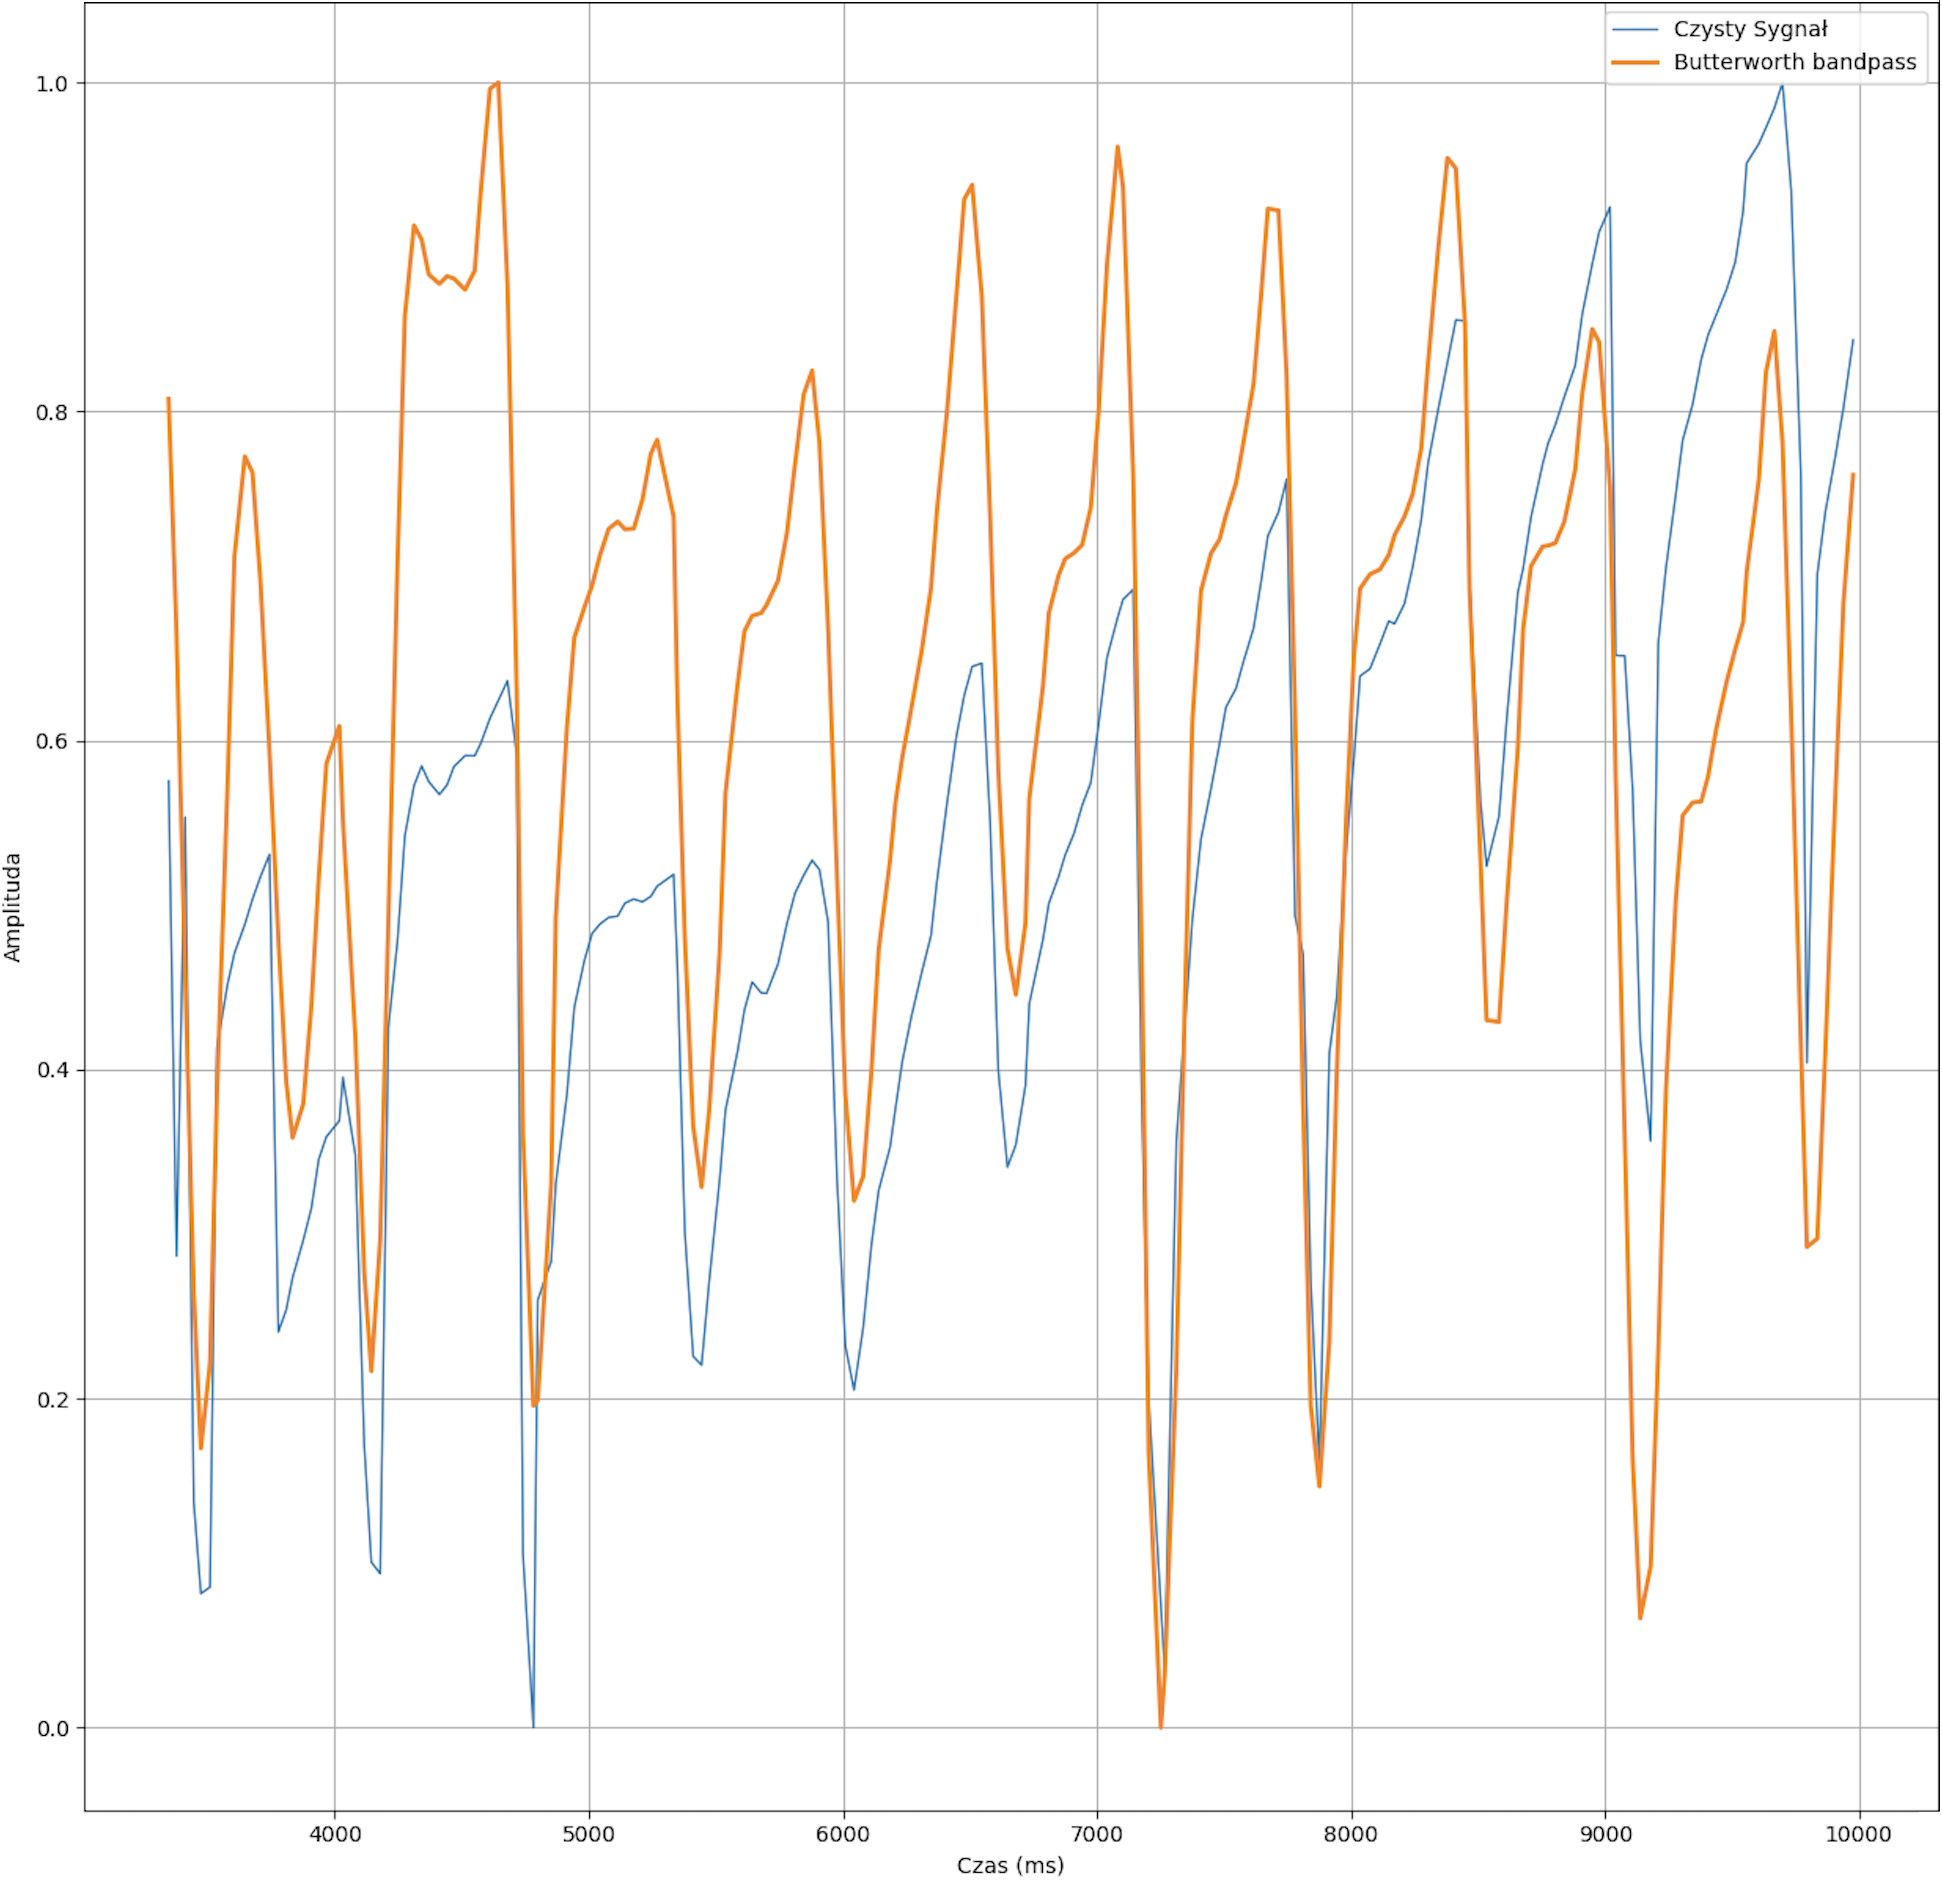
\includegraphics[width=0.76\linewidth]{Filtr_PPG.png} 
    \caption{A comparison between raw and filtered PPG signal}
    \label{fig:filtr_ppg}
\end{figure}

To improve PPG signal quality, a fourth-order digital filter with a frequency range of 0.5–5 Hz was employed. The lower cutoff frequency reduces interference caused by body movements or unstable detector placement, while the upper cutoff frequency attenuates device noise and optical artifacts \cite{26}. Signal filtration was implemented using the SciPy library, ensuring minimal phase distortion of the waveform.
%Dla poprawy jakości sygnału PPG wykorzystano filtr  czwartego rzędu, działający w zakresie 0,5–5 Hz. Dolna granica pasma ogranicza zakłócenia spowodowane ruchem ciała czy niestabilnym kontaktem czujnika ze skórą, natomiast górna tłumi szumy urządzenia pomiarowego i interferencje optyczne  \cite{26}. Filtracja została zrealizowana z wykorzystaniem  modułu SciPy, zapewniając obróbkę przebiegu bez przesunięcia fazowego.

%Modele detekcji
% Model do wykrywania załamków R
\newpage
\subsection{Detection models}
\subsubsection{R-Peak detection model}
A neural network combining convolutional and recurrent layers was developed for R-peak detection in ECG recordings. This network constitutes the first step in computing RR intervals and deriving heart rate variability (HRV) parameters. The model processes one-dimensional voltage signals divided into segments, with each segment containing 256 samples and serving as a basic unit for waveform analysis.
% Opracowano sieć neuronową łączącą warstwy splotowe i rekurencyjne, przeznaczoną do detekcji szczytów R w zapisie EKG. Stanowi ona pierwszy etap w wyznaczaniu interwałów RR i obliczaniu parametrów zmienności rytmu serca. Model przetwarza jednowymiarowe sygnały napięcia elektrycznego podzielone na fragmenty po 256 próbek, stanowiących podstawową jednostkę analizowanego przebiegu.

The convolutional portion of the network consists of four 1D convolutional layers, with their parameters summarized in Chart~\ref{tab:ecg_layers}. These layers are responsible for extracting features from the input signal and expanding its representation by increasing the number of channels from 16 to 256 using filters of sizes 3 and 5. Each convolution is followed by BatchNorm1d normalization and the nonlinear activation function LeakyReLU. Dimensionality reduction is performed using a MaxPooling1D operation with a kernel size of 2, which shortens the sequence from 256 to 16 samples along the time axis, increasing the model’s robustness to noise and interference. The resulting [128 × 16] matrix serves as input to a unidirectional LSTM. The LSTM output is then flattened and passed to a dense layer with 128 neurons, followed by a final block of 256 elements, each corresponding to a sample in the input signal. The output from the LSTM layer is processed by linear modules, propagating the extracted features into logit space. Each element of the output vector represents the probability of an R peak at the corresponding sample, enabling binary classification at every point in the waveform.
% Część splotowa sieci obejmuje cztery warstwy konwolucyjne 1D, których parametry zestawiono w Tabeli~\ref{tab:ecg_layers}. Warstwy te odpowiadają za ekstrakcję cech z sygnału wejściowego, rozszerzając jego reprezentację poprzez zwiększenie liczby kanałów od 16 do 128 za pomocą filtrów o rozmiarach 5 i 3. Dla każdego przekształcenia zastosowano normalizację BatchNorm1d oraz nieliniową funkcję aktywacji LeakyReLU. Redukcja wymiarowości jest realizowana za pomocą operacji MaxPooling1D z jądrem o rozmiarze 2, skracającej długość sekwencji z 256 do 16 próbek wzdłuż osi czasowej oraz zwiększającej odporność modelu na szum i zakłócenia. Wynikowa macierz o wymiarach [128 × 16] stanowi wejście dla jednokierunkowej LSTM. Otrzymany wektor jest spłaszczany i przekazywany do warstwy z 128 neuronami, a następnie do bloku końcowego zawierającego 256 elementów, reprezentujące kolejne próbki sygnału wejściowego. Dane wyjściowe z warstwy LSTM są  przetwarzane przez moduły liniowe, odwzorowujące wyekstrahowane cechy w przestrzeń logitów. Każdy element wektora odpowiada prawdopodobieństwu obecności szczytu R w danej próbce, umożliwiając binarną klasyfikację w każdym punkcie czasowym przebiegu. 

%Parametry bloków konwolucyjnych sieci
\begin{table}[h!]
\centering
\caption{Block parameters of convolutional networks}
\label{tab:ecg_layers}
\begin{tabular}{|l|c|c|c|c|c|}
\hline
\textbf{Block} & \textbf{In.} & \textbf{Out.} & \textbf{Filter} & \textbf{Padding} & \textbf{Act./Norm.} \\
\hline
Conv1D-1 & 1   & 16  & 5 & 2 & LReLU+BN \\
Conv1D-2 & 16  & 32  & 5 & 2 & LReLU+BN \\
Conv1D-3 & 32  & 64  & 3 & 1 & LReLU+BN \\
Conv1D-4 & 64  & 128 & 3 & 1 & LReLU+BN \\
\hline
\end{tabular}
\end{table}

Model was trained in a supervised mode based on the signals acquired from Polar H10 detector. Actual R peaks in a filtered ECG record have been computed using the Pan-Tompkins algorithm based on multi-step processing. The first phase is band-pass suppression of low and high frequency distortionary components. Waveform differentiation enhances steep curves of QRS complex. Afterwords a square of an average value of all samples in a moving integrating window is being computed. The final peak detection is realized using analysis of the integrated curve and local maximums \cite{27}.
Each point is assigned a binary label identifying the presence or absence of an extrema. Labels when then used for pattern classification corresponding to actual R peaks.
\newpage
Learning process was performed in mini-batches of 32 elements using the BCEWithLogitsLoss loss function. Adam algorithm was used for optimization with a constant learning rate of 0.0001. The efficiency of the developed neural network has been assessed based on the results obtained from an independent dataset using the model's trained parameters. Classification results are presented as a confusion matrix in Chart~\ref{tab:conf_matrix}.
%Model wytrenowano w trybie nadzorowanym na podstawie sygnałów pozyskanych z czujnika Polar H10. Rzeczywiste załamki R w przefiltrowanym zapisie EKG wyznaczono algorytmem Pan–Tompkinsa opartym na wieloetapowym przetwarzaniu. Początkową fazą jest pasmowo-przepustowe tłumienie składowych zakłócających o niskiej oraz wysokiej częstotliwości. Różniczkowanie przebiegu uwydatnia strome zbocza zespołu QRS, następnie obliczana jest średnia wartość próbek podniesionych do kwadratu w ruchomym oknie całkującym. Ostateczna detekcja szczytów jest realizowana poprzez progowanie zintegrowanej krzywej oraz analizę lokalnych maksimów \cite{27}.
%Każdemu punktowi przypisano etykietę binarną wskazującą obecność lub brak ekstremum, umożliwiając sieci klasyfikację wzorców odpowiadających rzeczywistym pikom R. 
%\newpage
%Proces uczenia przeprowadzono w partiach po 32 elementy z wykorzystaniem funkcji straty BCEWithLogitsLoss. Do optymalizacji zastosowano algorytm Adam przy stałej wartości learning rate wynoszącej 0,0001. Efektywność zaprojektowanej sieci neuronowej oceniono na podstawie wyników uzyskanych na niezależnym zbiorze danych, wykorzystując wytrenowane parametry modelu. Rezultaty klasyfikacji przedstawiono w postaci macierzy konfuzji w Tabeli~\ref{tab:conf_matrix}.


\begin{table}[ht]
\centering
\caption{Confusion matrix for R peak detection}
\label{tab:conf_matrix}
\begin{tabular}{|c|c|c|}
\hline
\textbf{Actual / Prediction} & \textbf{No peak } & \textbf{Peak } \\
\hline
No peak  & 231170 & 53 \\
Peak  & 83 & 2678 \\
\hline
\end{tabular}
\end{table}

A total of 231170 samples not containing an R peak and 2678 samples with actual R peaks were correctly classified by the model. The number of false positive predictions totaled 53, while the number of false negatives was 83. The F1 score of 0.9753 indicates a good balance between precision and sensitivity, which is a key feature in automated electrocardiographic signal analysis. Basic quality assessment metrics are presented in Chart~\ref{tab:metrics}.
%Model poprawnie zaklasyfikował 231170 próbek niezawierających piku R oraz 2678 z jego rzeczywistą obecnością. Liczba fałszywie pozytywnych predykcji wyniosła 53, natomiast fałszywie negatywnych -- 83. Wartość miary F1 równa 0,9753 świadczy o wysokiej równowadze pomiędzy precyzją a czułością modelu, co jest kluczowe w automatycznej analizie sygnałów elektrokardiograficznych. Podstawowe metryki oceny jakości modelu przedstawiono w Tabeli~\ref{tab:metrics}.

\begin{table}[ht]
\centering
\caption{R peak detection parameters}
\label{tab:metrics}
\begin{tabular}{|c|c|p{4.6cm}|}
\hline
\textbf{Metric} & \textbf{Value} & \textbf{Description} \\
\hline
Efficiency & 96,99\% & A percentage of correct classifications of R peaks or lack thereof. \\
Incorrect detections & 0,00\% & A percentage of samples falsely classified as containing R peaks. \\
Skipped peaks & 3,01\% & A percentage of samples with undetected actual R peaks. \\
\hline
\end{tabular}
\end{table}

%Model do wykrywania szczytów fali
\subsubsection{Wave peak detection model}
Analogous to the approach applied in ECG signal analysis, a convolutional model for identifying local peaks in the photoplethysmographic waveform was developed. This model forms the basis for determining inter-beat intervals (IBIs) used to estimate heart rate parameters. The network processes data as a single-channel vector containing 50 samples, with each sample representing changes in blood volume within the vessels.
%Analogicznie do podejścia zastosowanego w analizie sygnału EKG, opracowano model konwolucyjny identyfikujący lokalne szczyty w przebiegu fotopletyzmograficznym. Stanowi on podstawę do wyznaczania interwałów międzyuderzeniowych IBI, wykorzystywanych przy estymacji wskaźników rytmu serca. Sieć przetwarza dane w postaci wektora zawierającego 50 próbek w pojedynczym kanale, reprezentujących zmiany objętości krwi w naczyniach obwodowych.

A one-dimensional convolutional layer with 32 filters, each 7 samples wide, complemented by BatchNorm1d normalization and the GELU activation function, constitutes the first element of the architecture. The purpose of the activation function is to increase the stability of the learning process while providing gentle non-linearity. The next four residual blocks process local signal patterns. The first block increases the number of channels from 32 to 64 using a kernel of size 9. The following block expands the number of channels from 64 to 128 with a kernel width of 5 samples. The remaining two blocks maintain the same depth while using filters of sizes 3 and 7, respectively. The initial transformations are followed by a Dropout layer to reduce overfitting.
\newpage
The SE module increases the model’s selectivity, improving the accuracy of local waveform peak detection. A convolutional block with a kernel size of 1 compresses the number of channels from 128 to 64, while two fully connected linear layers reduce the dimensionality to 64 and 32, each followed by a GELU activation function. The resulting one-dimensional output vector is passed through a Sigmoid function, allowing the values to be interpreted as probabilities of local peaks in the PPG signal. Detailed block parameters are provided in Chart~\ref{tab:ppg_layers}.
%Pierwszy element architektury stanowi jednowymiarowa warstwa splotowa z 32 filtrami o szerokości 7 próbek, uzupełniona normalizacją BatchNorm1d oraz funkcją aktywacji GELU, odpowiedzialną za łagodną nieliniowość i poprawę stabilność procesu uczenia. Cztery kolejne bloki resztkowe przetwarzają lokalne wzorce sygnału. Pierwszy moduł zwiększa kanały z 32 do 64, wykorzystując jądro o rozmiarze 9.  Rozszerzenie liczby wymiarów z 64 do 128 realizuje segment przy zastosowaniu okna o długości 5 próbek, natomiast dwa pozostałe utrzymują tę samą głębokość, operując filtrami o wielkości 3 i 7. Transformacje zdefiniowane w początkowym etapie zostały rozszerzone o warstwę Dropout, umożliwiającą redukcję nadmiernego dopasowania. 
%\newpage
%Moduł SE podnosi selektywność modelu, poprawiając precyzję wykrywania lokalnych maksimów przebiegu. Kompresję kanałów z 128 do 64 zapewnia blok konwolucyjny z jądrem o rozmiarze 1, a dwie w pełni połączone operacje liniowe zmniejszają wymiary do 64 i 32, z funkcją aktywacji GELU. Jednowymiarowy wektor wyjściowy podlega transformacji Sigmoid, umożliwiając interpretację wartości jako prawdopodobieństwo lokalnych szczytów w zapisie PPG. Szczegółowe parametry bloków uwzględniono w Tabeli~\ref{tab:ppg_layers}.

%Parametry bloków konwolucyjnych sieci
\begin{table}[ht]
\centering
\caption{Convolutional network's block parameters}
\label{tab:ppg_layers}
\begin{tabular}{|l|c|c|c|c|c|}
\hline
\textbf{Block} & \textbf{In.} & \textbf{Out.} & \textbf{Filter} & \textbf{Padding} & \textbf{Act./Norm.} \\
\hline
Conv1D & 1 & 32 & 7 & 3 & GELU+BN \\
ResidualBlock 1 & 32 & 64 & 9 & 4 & GELU+BN+DO \\
ResidualBlock 2 & 64 & 128 & 5 & 2 & GELU+BN+DO \\
ResidualBlock 3 & 128 & 128 & 3 & 1 & GELU+BN+DO\\
ResidualBlock 4 & 128 & 128 & 7 & 3 & GELU+BN+DO \\
SEBlock & 128 & 128 & – & – & SE scaling \\
Conv1D  & 128 & 64 & 1 & 0 & GELU+BN \\
FC & 128 & 64 & – & – & GELU \\
FC & 64 & 32 & – & – & GELU \\
Output & 32 & 1 & – & – & Sigmoid \\
\hline
\end{tabular}
\end{table}

The supervised learning process for PPG data was performed on signal segments acquired from a mobile device, which were preprocessed using filtration and normalized to the range [-1, 1]. Each segment was assigned a vector of binary labels indicating the presence or absence of a peak. These labels were derived from local peak identification, where a peak is defined as a value exceeding its neighboring samples, allowing classification within the window. The network was trained on 50-sample waveform fragments in mini-batches of 32, using the BCELoss function and the Adam optimizer with a constant learning rate of 0.001. The performance of the developed model was evaluated on an independent dataset using the parameters obtained during training. Classification results are presented as a confusion matrix in Chart~\ref{tab:conf_matrix_ppg}.
%Proces uczenia nadzorowanego dla danych PPG przeprowadzono na segmentach sygnału pochodzących z urządzenia mobilnego, poddanych wstępnej filtracji i normalizacji do zakresu [-1, 1]. W każdym wycinku przypisano wektor etykiet binarnych określający obecność lub brak piku, oparty na identyfikacji lokalnych szczytów przewyższających sąsiednie wartości, umożliwiając klasyfikację wzorców w obrębie okna. Sieć trenowano na 50-punktowych fragmentach przebiegu, w partiach po 32 segmenty, wykorzystując funkcję straty BCELoss oraz optymalizator Adam ze stałym współczynnikiem uczenia równym 0,001. Skuteczność zaprojektowanego modelu oceniono na podstawie wyników uzyskanych na niezależnym zbiorze danych, przy zastosowaniu parametrów wyznaczonych podczas dopasowania. Wyniki klasyfikacji przedstawiono w formie macierzy konfuzji w Tabeli~\ref{tab:conf_matrix_ppg}.

%Macierz konfuzji dla detekcji pików fali
\begin{table}[ht]
\centering
\caption{Confusion matrx for wave peaks detection}
\label{tab:conf_matrix_ppg}
\begin{tabular}{|c|c|c|}
\hline
\textbf{Actual / Prediction} & \textbf{No peak } & \textbf{Peak} \\
\hline
No peak  & 9609 & 9 \\

Peak  & 7 & 375 \\
\hline
\end{tabular}
\end{table}

% TODO:(mati): miara F1 -> F1 benchmark?
For photoplethysmographic signals, the network correctly identified 375 samples containing a wave peak and 9609 samples without one. Incorrect predictions included 9 false positives and 7 false negatives. The obtained F1 score of 0.9774 is comparable to that of the ECG model, confirming the validity of the applied approach for analyzing both signal types. Basic quality assessment metrics for the architecture are presented in Chart~\ref{tab:metrics_ppg}.
%Dla sygnałów fotopletyzmograficznych sieć poprawnie rozpoznała 9609 próbek bez obecności fali oraz 375 z jej wystąpieniem. Niepoprawne predykcje odnotowano w 9 przypadkach fałszywie dodatnich oraz 7  fałszywie ujemnych. Otrzymana wartość miary F1, wynosząca 0,9774, jest zbliżona do wyników uzyskanych dla modelu EKG, potwierdzając wiarygodność zastosowanego rozwiązania w analizie obu typów sygnałów.
%Podstawowe metryki oceny jakości architektury przedstawiono w Tabeli~\ref{tab:metrics_ppg}.

%Parametry detekcji szczytów fali
\begin{table}[ht]
\centering
\caption{Wave peak detection parameters}
\label{tab:metrics_ppg}
\begin{tabular}{|c|c|p{4.6cm}|}
\hline
\textbf{Metric} & \textbf{Value} & \textbf{Description} \\
\hline
Efficiency & 98,17\% & Percentage of correctly classified samples. \\
Incorrect detections & 0,52\% & Percentage of samples falsely classified as containing the wave peak. \\
Skipped peaks & 1,83\% & Percentage of sample with undetected actual wave peak. \\
\hline
\end{tabular}
\end{table}

%Ewaluacja maksimów i analiza czasowa sygnałów biomedycznych
%Weryfikacja skuteczności detekcji pików R
\newpage
\section{Maxima evaluation and time analysis of biomedical signals}
\subsection{R peak detection efficiency verification}
The performance of the convolutional network architecture for R peak detection in electrocardiographic signals was evaluated against the classic Pan-Tompkins algorithm and reference R peaks obtained using the NeuroKit library, which serves as a gold standard. The signal was sampled at 130 Hz and processed in overlapping segments containing 256 samples.
%Skuteczność architektury opartej na sieci splotowej w wykrywaniu pików R w zapisie elektrokardiograficznym oceniono względem klasycznego algorytmu Pan–Tompkinsa oraz szczytów referencyjnych uzyskanych w ramach biblioteki NeuroKit, pełniącej rolę złotego standardu. Sygnał próbkowano z częstotliwością 130 Hz i przetwarzano w niepokrywających się segmentach obejmujących 256 próbek. 

The total number of detected maxima was 54 for the model, 56 using the Pan-Tompkins method, and 56 for the reference data. The results are presented in Chart~\ref{tab:peak_comparison}, showing the number of True Positives, False Positives, and False Negatives, as well as the computed precision, sensitivity, and F1 scores, with a tolerance corresponding to 1–2 waveform samples.
% Łączna wartość wykrytych maksimów wyniosła 54 dla modelu, 56 metodą Pan-Tompkinsa oraz 56 w danych wzorcowych. Wyniki przedstawiono w Tabeli~\ref{tab:peak_comparison}, zawierającej liczbę prawdziwych trafień TP, fałszywych alarmów FP, pominiętych szczytów FN, wraz z obliczonymi wskaźnikami precyzji, czułości i F1, przy tolerancji odpowiadającej 1–2 punktom przebiegu.

%Ocena technik wyznaczania ekstremów
\begin{table}[ht]
\caption{Extrema detecting techniques assessment}
\label{tab:peak_comparison}
\centering
\begin{tabular}{|p{3.08cm}|c|c|c|c|c|c|}
\hline
\textbf{Method} & \textbf{TP} & \textbf{FP} & \textbf{FN} & \textbf{Prec.} & \textbf{Sens.} & \textbf{F1} \\
\hline
AI vs Pan-Tompkins & 54 & 0 & 2 & 1.000 & 0.964 & 0.982 \\
AI vs NeuroKit & 53 & 1 & 3 & 0.981 & 0.946 & 0.964 \\
Pan-Tompkins vs NeuroKit & 55 & 1 & 1 & 0.982 & 0.982 & 0.982 \\
\hline
\end{tabular}
\end{table}

\begin{figure}[htbp]
    \centering
    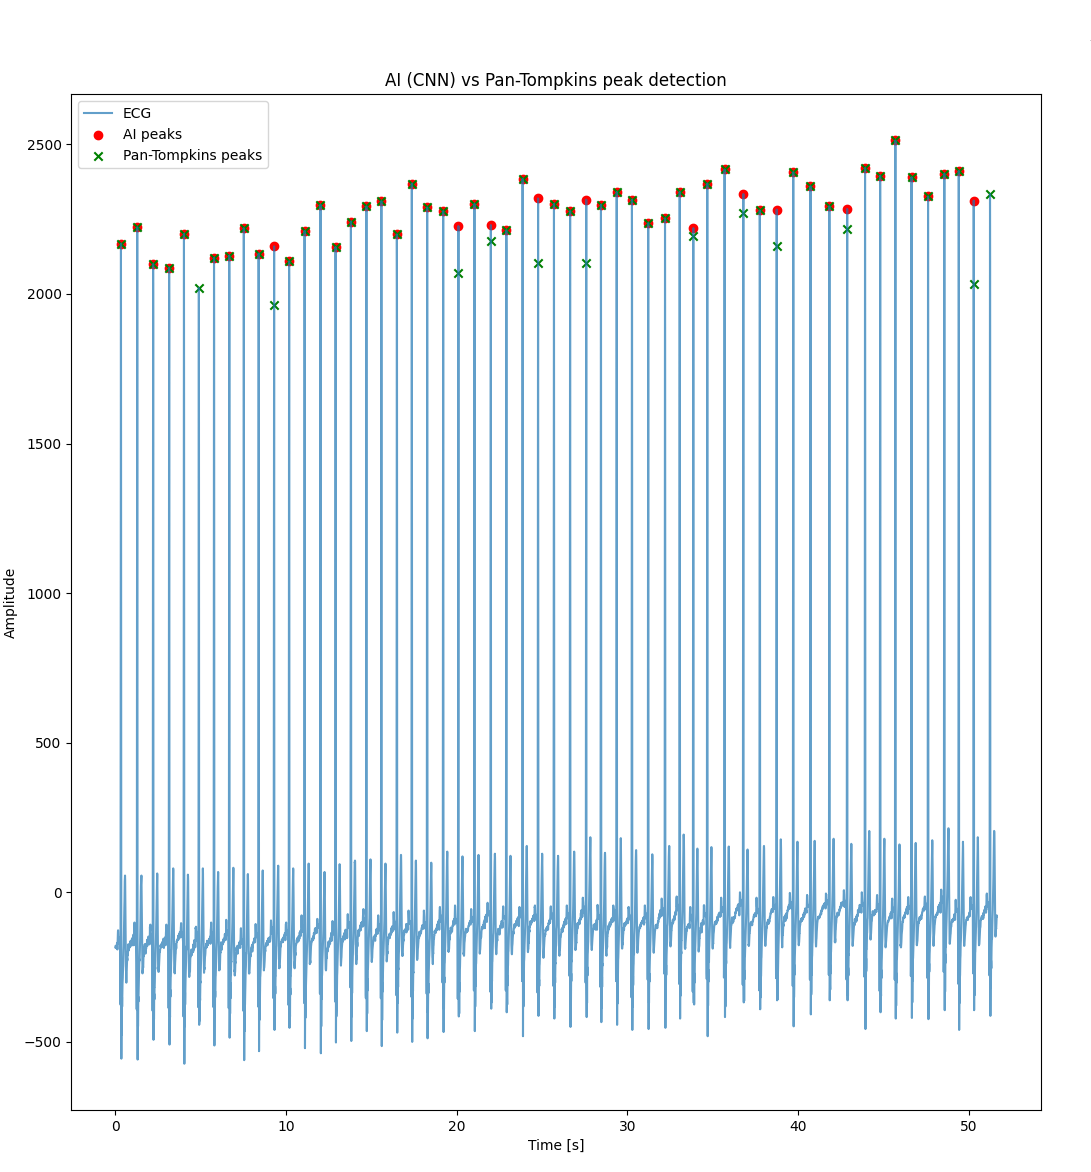
\includegraphics[scale=0.2]{ai_pan-tompkins.png}
    \caption{Comparison of R peak detection between the network and Pan-Tompikns algorithm}
    \label{fig:ai_pan-tompkins}
\end{figure}

\begin{figure}[htbp]
    \centering
    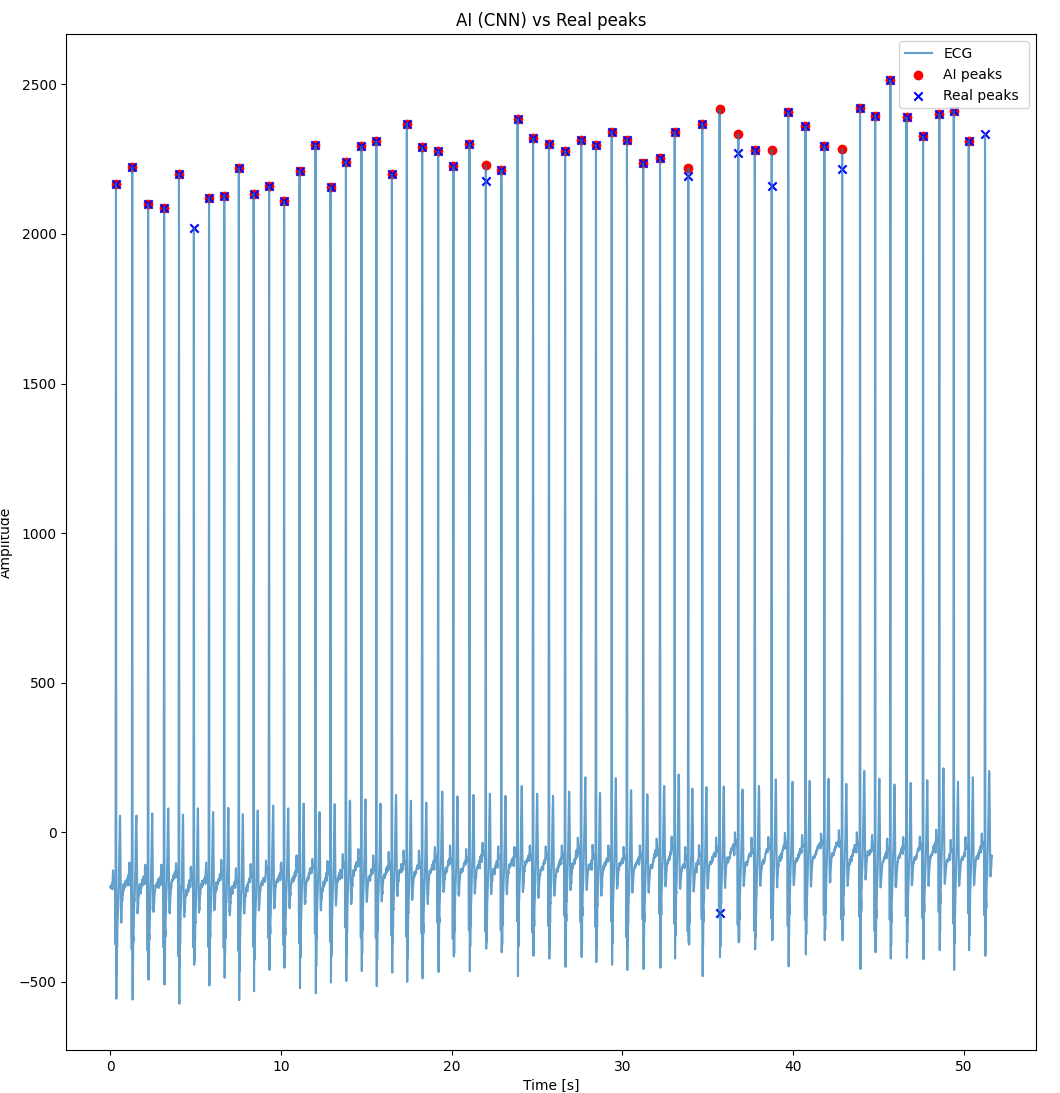
\includegraphics[scale=0.2]{ai_real_peaks.png}
    \caption{Comparison of R peak detection between the network and reference peaks}
    \label{fig:ai_real_peaks}
\end{figure}


\newpage
The network’s performance in detecting R peaks is comparable to the classic Pan-Tompkins algorithm and shows high agreement with the reference values. Discrepancies resulting from missed or shifted peaks can be reduced through optimized signal preprocessing or further model training. Current machine learning systems are capable of achieving high performance in the automated detection of local peaks in electrocardiographic signals.
%Skuteczność sieci w wykrywaniu pików R jest porównywalna z klasycznym algorytmem Pan-Tompkinsa i charakteryzuje się wysoką zgodnością z wartościami referencyjnymi. Rozbieżności wynikające z pominiętych lub przesuniętych ekstremów można zredukować poprzez optymalizację wstępnej obróbki sygnału lub dalsze trenowanie modelu. Obecne systemy uczenia maszynowego wykazują zdolność do osiągania niemal najwyższej klasy skuteczności w automatycznym wykrywaniu lokalnych szczytów zapisu elektrokardiograficznego.

%Weryfikacja skuteczności detekcji pików fali
\subsection{Wave peak detection efficiency verification}
Peak identification in photoplethysmographic waveforms was performed using the convolutional network and a reference signal obtained through band-pass filtering and local maximum detection. The data were divided into segments of 100 samples each and normalized to the range [-1, 1]. In windowed mode, the model predictions were converted into point indices corresponding to potential wave peaks.
%Identyfikacje szczytów przebiegu fotopletyzmograficznego przeprowadzono na podstawie wyników sieci konwolucyjnej oraz sygnału referencyjnego uzyskanego metodą filtracji pasmowo-przepustowej i lokalnego wyszukiwania maksimów. Dane podzielono na segmenty o długości 100 próbek i znormalizowano do zakresu [−1,1]. W trybie okienkowym predykcje modelu przekształcono w indeksy punktów odpowiadających potencjalnym pikom fali.

The machine learning algorithm detected 76 peaks, while the reference set contained 72. Detection performance was evaluated within a tolerance window of 264 ms, corresponding to 8 time units at a sampling rate of 30 Hz, using True Positive, False Positive, and False Negative metrics. The model produced 61 TP, 15 FP, and 11 FN, resulting in a precision of 0.803, a sensitivity of 0.847, and an F1 score of 0.824.
% Algorytm uczenia maszynowego wykrył 76 szczytów, natomiast zestaw wzorcowy obejmował 72. Skuteczność detekcji przebiegła w przedziale tolerancji 264 ms, odpowiadającym 8 jednostkom czasowym przy częstotliwości próbkowania 30 Hz, z zastosowaniem parametrów prawdziwych trafień TP, fałszywych alarmów FP oraz pominiętych pików FN. Model uzyskał 61 TP, 15 FP oraz 11 FN, przekładając się na precyzję 0,803, czułość 0,847 oraz miarę F1 równą 0,824.

%Porównanie detekcji pików fali przez sieć splotową z szczytami referencyjnymi
\begin{figure}[htbp]
    \centering
    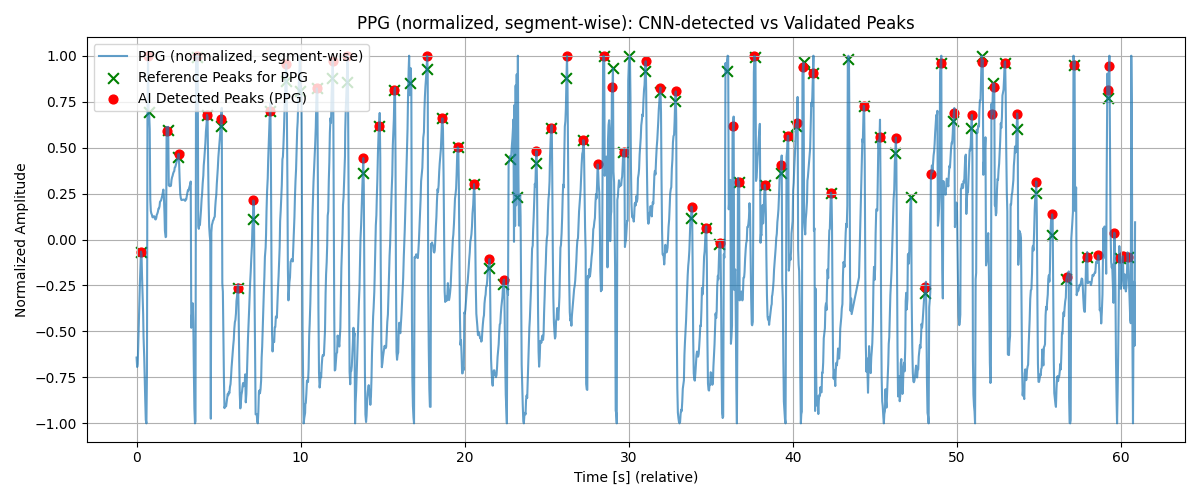
\includegraphics[scale=0.28]{ppg_ai_vs_real.png}
    \caption{Peak detection comparison between the convolutional network and reference peaks}
    \label{fig:ppg_ai_real_peaks}
\end{figure}

\newpage
The results indicate a high agreement between the network and the reference photoplethysmographic waveform maxima. The low number of false detections was primarily due to interferences and limitations of short-segment analysis. These results suggest the practical utility of the network in digital biomedical signal processing.
%Wyniki wskazują na wysoką zgodność architektury z referencyjnymi maksimami przebiegu fotopletyzmograficznego, przy niewielkiej liczbie fałszywego wykrywania spowodowanego zakłóceniami i ograniczeniami analizy krótkich segmentów. Uzyskane rezultaty sugerują praktyczną użyteczność sieci w cyfrowym przetwarzaniu sygnałów biomedycznych.


%Estymacja PTT ze zsynchronizowanych sygnałów
\subsection{PTT estimation from the synchronized signals}
Different timestamp schemes are used during ECG and PPG recordings. In electrocardiography, R peak occurrences are defined relative to the start of acquisition and saved in seconds as relative time. During data processing, these values are converted to absolute UNIX time, allowing comparison with the PPG waveform. In photoplethysmography, wave peak detection is recorded directly using the system time.
%Podczas rejestracji sygnałów EKG i PPG wykorzystywane są różne schematy zapisu znaczników czasowych. W elektrokardiogramie punkty wystąpienia załamków R początkowo określane są względem chwili rozpoczęcia akwizycji i zapisywane w sekundach jako czas względny. Podczas przetwarzania danych wartości te są przekształcane do formatu absolutnego UNIX, umożliwiając porównanie z przebiegiem PPG. W fotopletyzmografii detekcja szczytów fali rejestrowana jest bezpośrednio w czasie systemowym.

%Dla ujednolicenia układu czasowego przekształca się dane EKG z czasu względnego na znaczniki UNIX, zgodnie z równaniem (2):
To unify the time systems, ECG data are converted from relative time to UNIX timestamps according to Equation (2).
\begin{equation}
t_{\mathrm{UNIX}} = t_{\mathrm{rel}} + t_{0},
\end{equation}
where $t_{\mathrm{UNIX}}$ - time in UNIX format, $t_{\mathrm{rel}}$ – relative time, a $t_{0}$ – beginning of the acquisition.

%Przebiegi zostały przedstawione w jednej osi czasu, umożliwiając ich automatyczną synchronizację. Dopasowanie par szczytów realizowano poprzez przypisanie do każdego załamka R w zapisie elektrokardiograficznym najbliższego w kolejności wystąpień ekstremum w sygnale fotopletyzmograficznym. Nie każdy zarejestrowany pik w EKG posiada odpowiadający punkt w PPG, wynikający z zakłóceń ruchowych lub utraty próbek. Różnice czasowe między dopasowanymi maksimami definiowane są jako interwał propagacji tętna PTT, wyznaczany zgodnie z równaniem (3):
Waveforms are presented on a single time axis, enabling their automatic synchronization. Peak pairing is performed by assigning each R peak in the electrocardiographic record to the closest extremum in order of occurrence from the photoplethysmographic signal. Not every recorded ECG peak has a corresponding PPG peak, which can be attributed to movement interferences or sample loss. Time differences between matched maxima are defined as the PTT (Pulse Transit Time) and are computed according to Equation (3).
\begin{equation}
PTT = t_{\mathrm{PPG}} - t_{\mathrm{ECG}},
\end{equation}
where $t_{\mathrm{PPG}}$, $t_{\mathrm{ECG}}$ - PPG and ECG peak detection moments. 

\newpage
\begin{figure}[htbp]
    \centering
    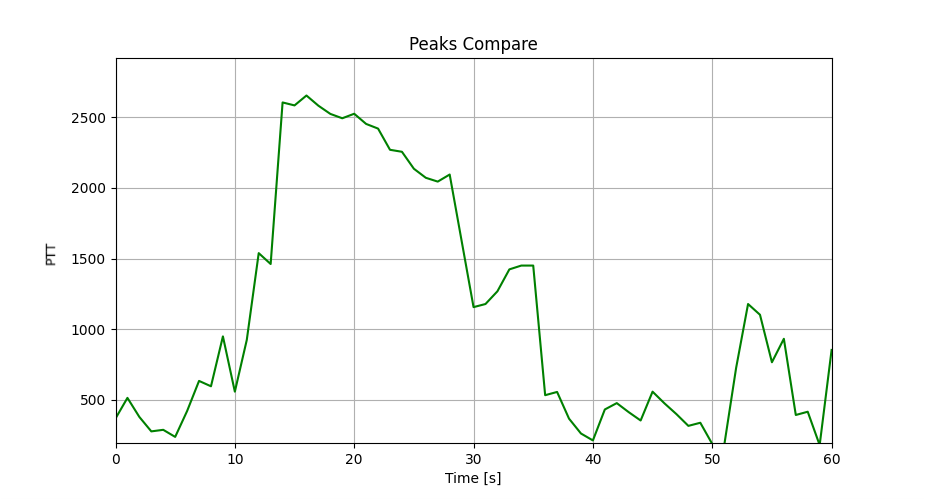
\includegraphics[width=1.0\linewidth]{Peaks_compare.png}
   \caption{Time differences between ECG and PPG peaks}%Chwilowe różnice czasowe między szczytami EKG i PPG
    \label{fig:PTT}
\end{figure}

%Z wektora wartości wyznacza się statystyki opisowe, obejmujące średnią, określającą przeciętny czas przejścia fali tętna, oraz odchylenie standardowe, wyrażające jego zmienność.
Descriptive statistics were computed from the value vector, including the mean, which defines the average time of the heart rate phase shift, and the standard deviation, which represents its variability.

%Wskaźniki HRV
\subsection{HRV indicators}
Gaps between consecutive heartbeats were analyzed independently in both signals. Relative time was used in electrocardiography, resulting from windowed processing of the samples, whereas in the photoplethysmography system, timestamps were employed to ensure consistency with the recorded waveform and to allow synchronization with different data sources. RR intervals were determined from the ECG recordings, corresponding to the distances between R peaks. For PPG, IBI (Inter-Beat Interval) distances were computed. Based on these values, standard HRV parameters were calculated in RR form, and analogous calculations were performed for IBI.
%Odstępy między kolejnymi uderzeniami serca analizowano niezależnie w obu sygnałach. W elektrokardiografii wykorzystano czas względny, wynikający z okienkowego trybu przetwarzania próbek, natomiast w fotopletyzmografii zastosowano znaczniki systemowe, zapewniając spójność z rejestrowanym przebiegiem oraz umożliwiając synchronizację z innymi źródłami danych. Dla zapisu EKG określono interwały RR, odpowiadające odległościom między załamkami R, a w PPG odstępy międzyuderzeniowe IBI. Na podstawie tych wartości wyznaczono standardowe parametry HRV, przedstawione w formie RR. Analogiczne obliczenia przeprowadzono dla IBI.

\noindent\textit{1) Average interval length:} 
Arithmetic mean of RR intervals expressed with the Formula (4):
\begin{equation}
    Mean = \frac{1}{N} \sum_{i=1}^{N} RR_i
\end{equation}
where $RR_i$ -- $i$-th RR interval, and $N$ – analyzed interval count.

\noindent\textit{2) NN intervals standard deviation:} 
Total heart rate variability value, calculated based on all RR intervals expressed with the Formula (5):%Wielkość całkowitej zmienności rytmu serca, obliczana na podstawie wszystkich interwałów RR, wyrażona wzorem (5):
\begin{equation}
    SDNN = \sqrt{\frac{1}{N-1} \sum_{i=1}^{N} (RR_i - Mean)^2}
\end{equation}
where $Mean$ – average interval length, $RR_i$ – $i$-th RR interval, a $N$ – analyzed interval count. 
\newpage
\noindent\textit{3) Square root of averaged squares of differences between subsequent NN intervals:} 
Benchmark used in short-term heart rate fluctuations assessment expressed with the Formula (6):
\begin{equation}
    RMSSD = \sqrt{\frac{1}{N-1} \sum_{i=1}^{N-1} (RR_{i+1} - RR_i)^2}
\end{equation}
where $RR_i$ -- $i$-th RR interval, a $N$ – analyzed interval count.

\begin{figure}[h]
    \centering
    \begin{subfigure}{0.47\textwidth}
        \centering
        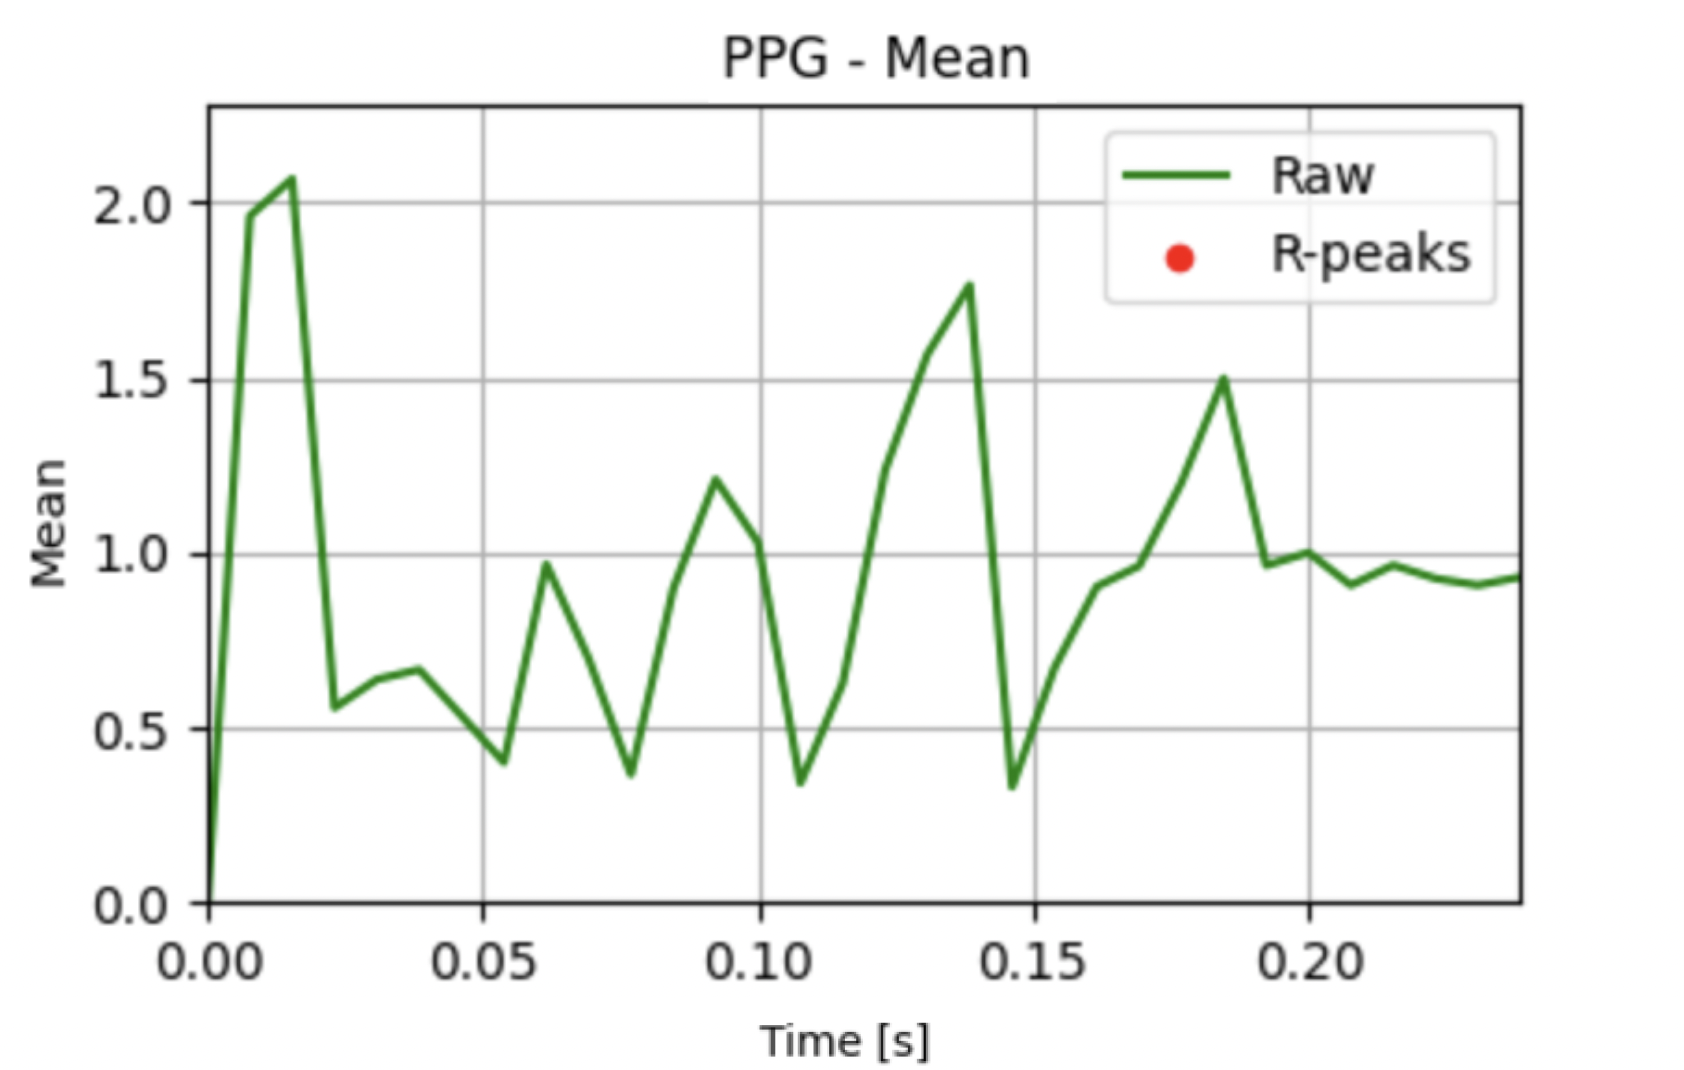
\includegraphics[width=\linewidth]{Mean.png}
        \caption{Average interval length}
    \end{subfigure}
    
   \vspace{0.2cm} 
    \begin{subfigure}{0.47\textwidth}
        \centering
        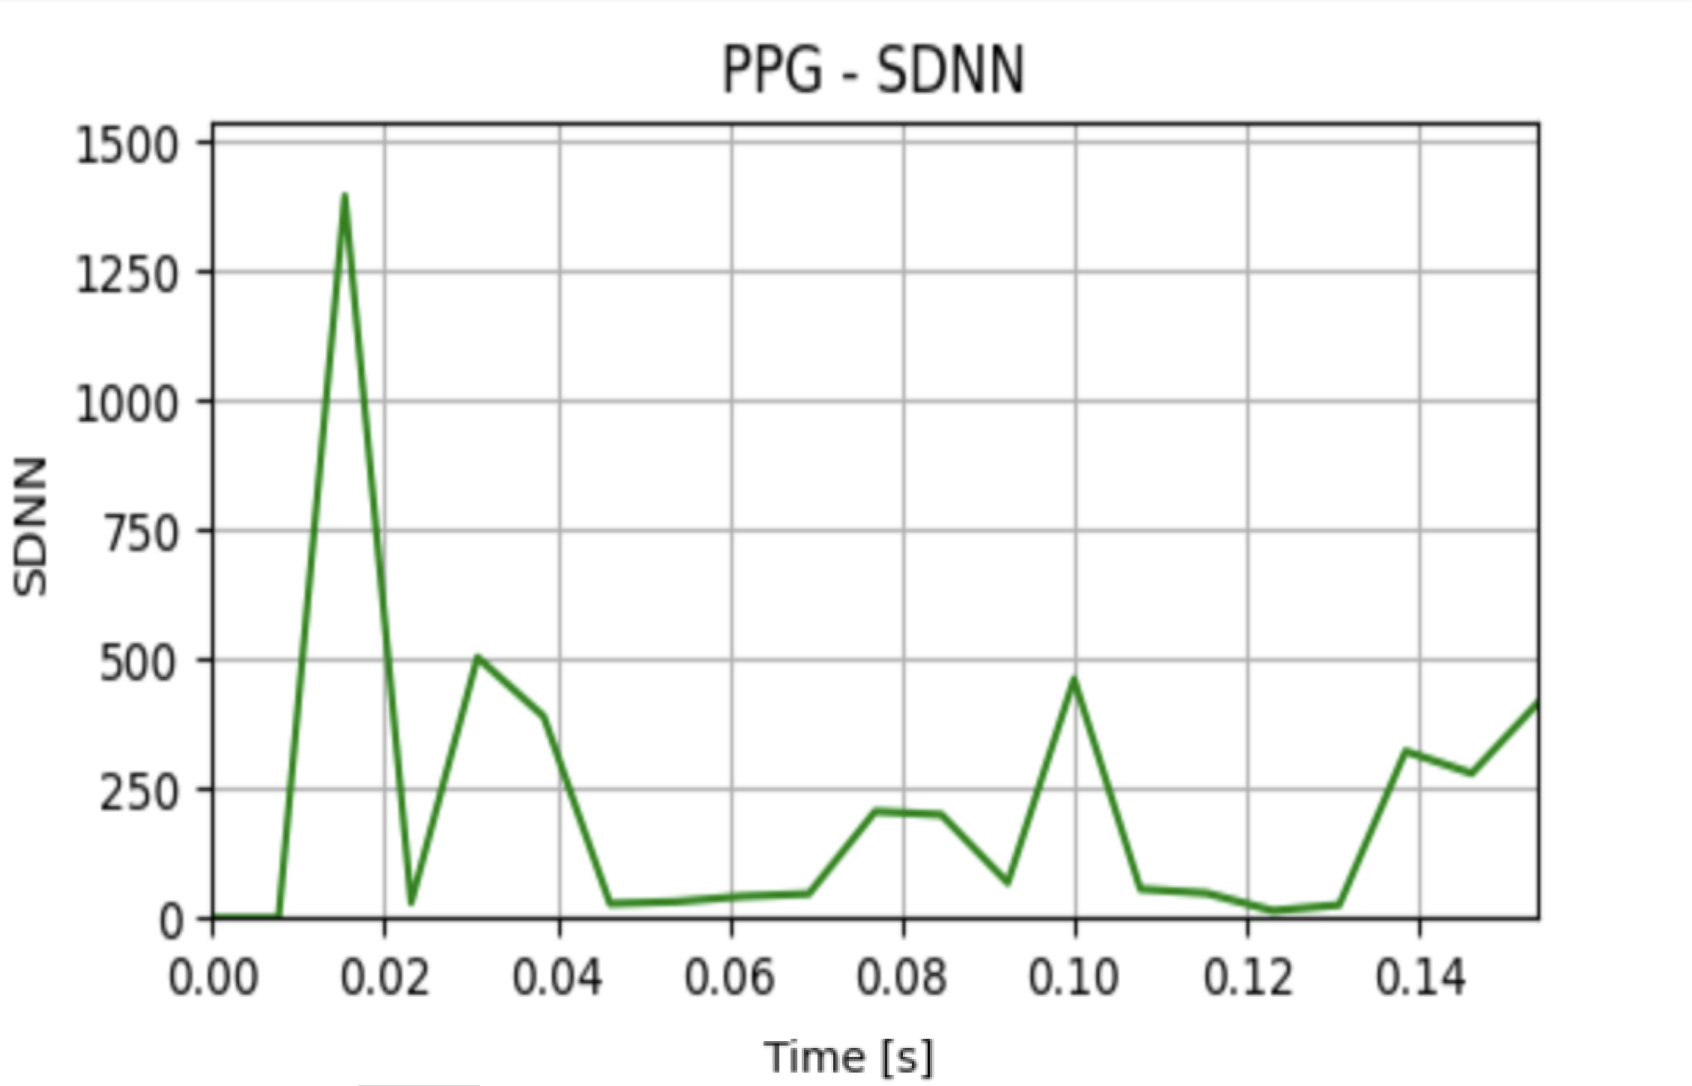
\includegraphics[width=\linewidth]{SDNN.png}
        \caption{Standard deviation of NN intervals}
    \end{subfigure}
    
    \vspace{0.2cm}  
    \begin{subfigure}{0.47\textwidth}
        \centering
        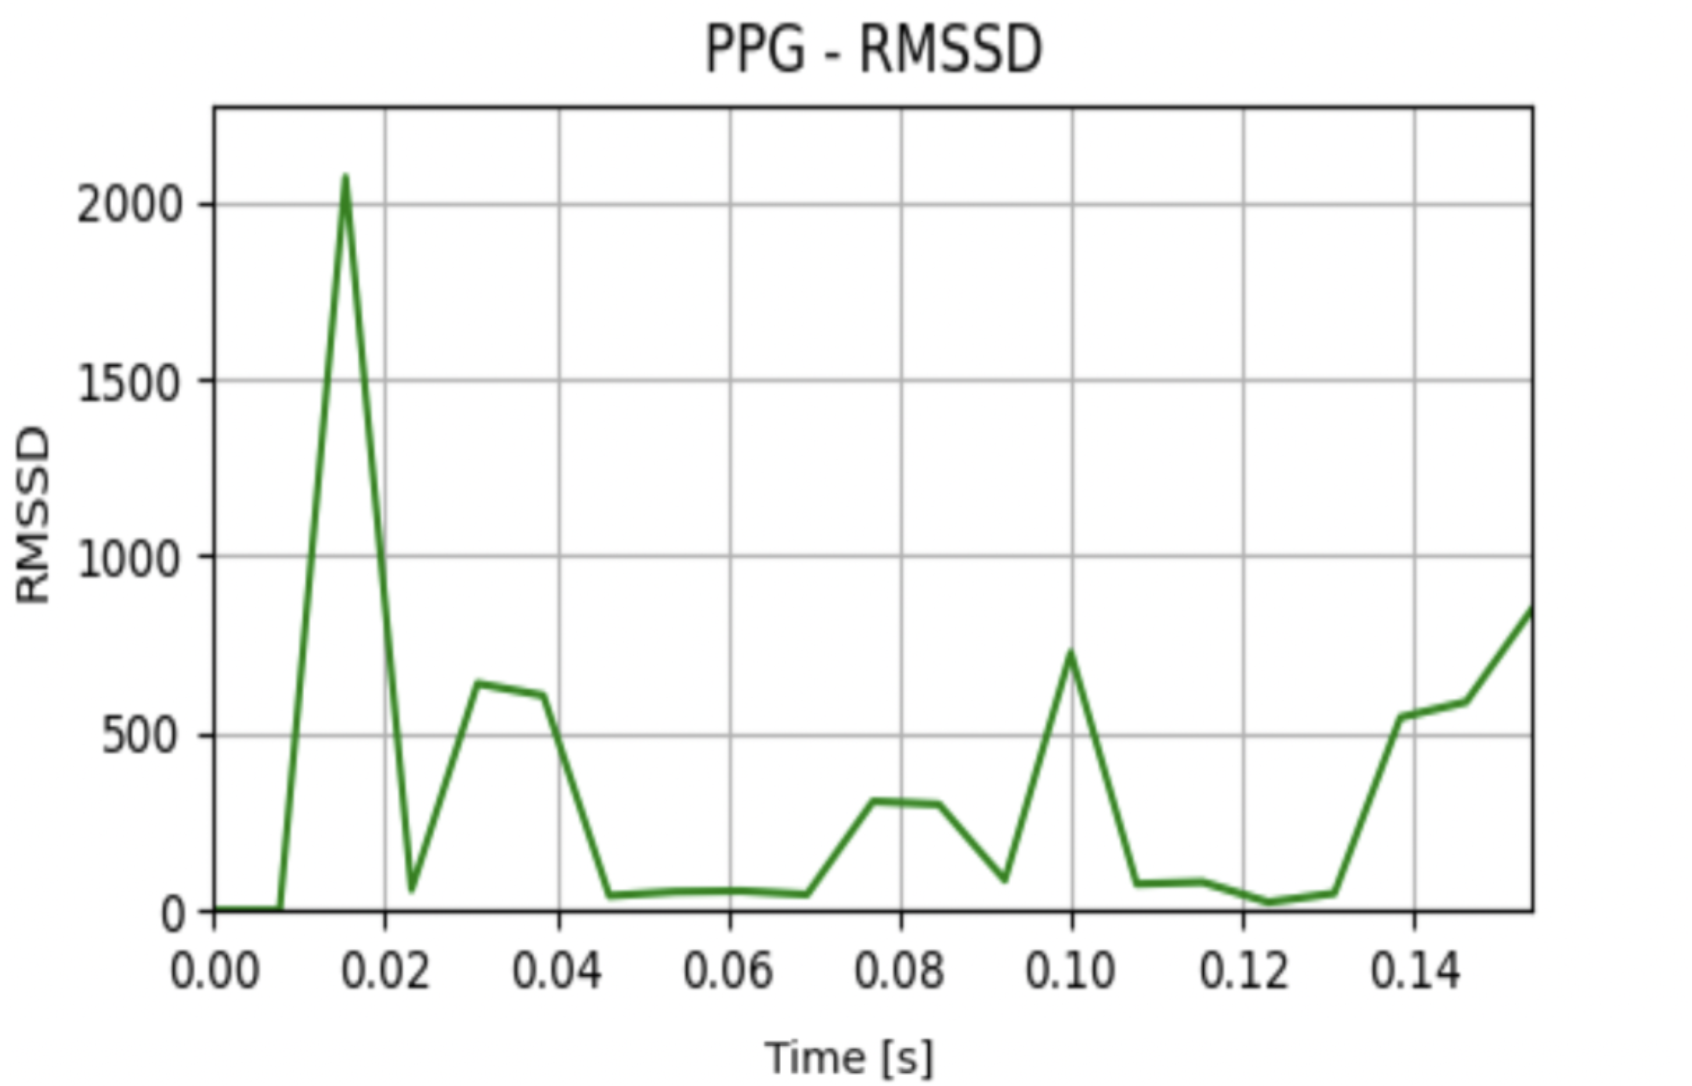
\includegraphics[width=\linewidth]{RMSSD.png}
        \caption{Square root of average of squares of differences}
    \end{subfigure}  
    \caption{Exemplary waveforms of HRV indicators computed for PPG}
\end{figure}

\newpage
A 60-second dynamic window was used for real-time processing. R peak markers and their corresponding intervals were updated online, while samples outside the window were discarded. SDNN, RMSSD, and average intervals between heartbeats were all presented as figures.
%Do obliczeń w czasie rzeczywistym wykorzystano dynamiczne okno o długości 60 s. Oznaczenia pików oraz odpowiadające im odstępy są aktualizowane w trybie online, natomiast próbki spoza okna są usuwane. Parametry SDNN, RMSSD oraz średnie interwały między uderzeniami serca przedstawiono w postaci wykresów.
%Added na dole:::

For comparison, HRV indicator waveforms computed from ECG signals are also shown:
%Dla porównania przedstawiono również przebiegi wskaźników HRV wyznaczonych z sygnału EKG:

\begin{figure}[h]
    \centering
    \begin{subfigure}{0.47\textwidth}
        \centering
        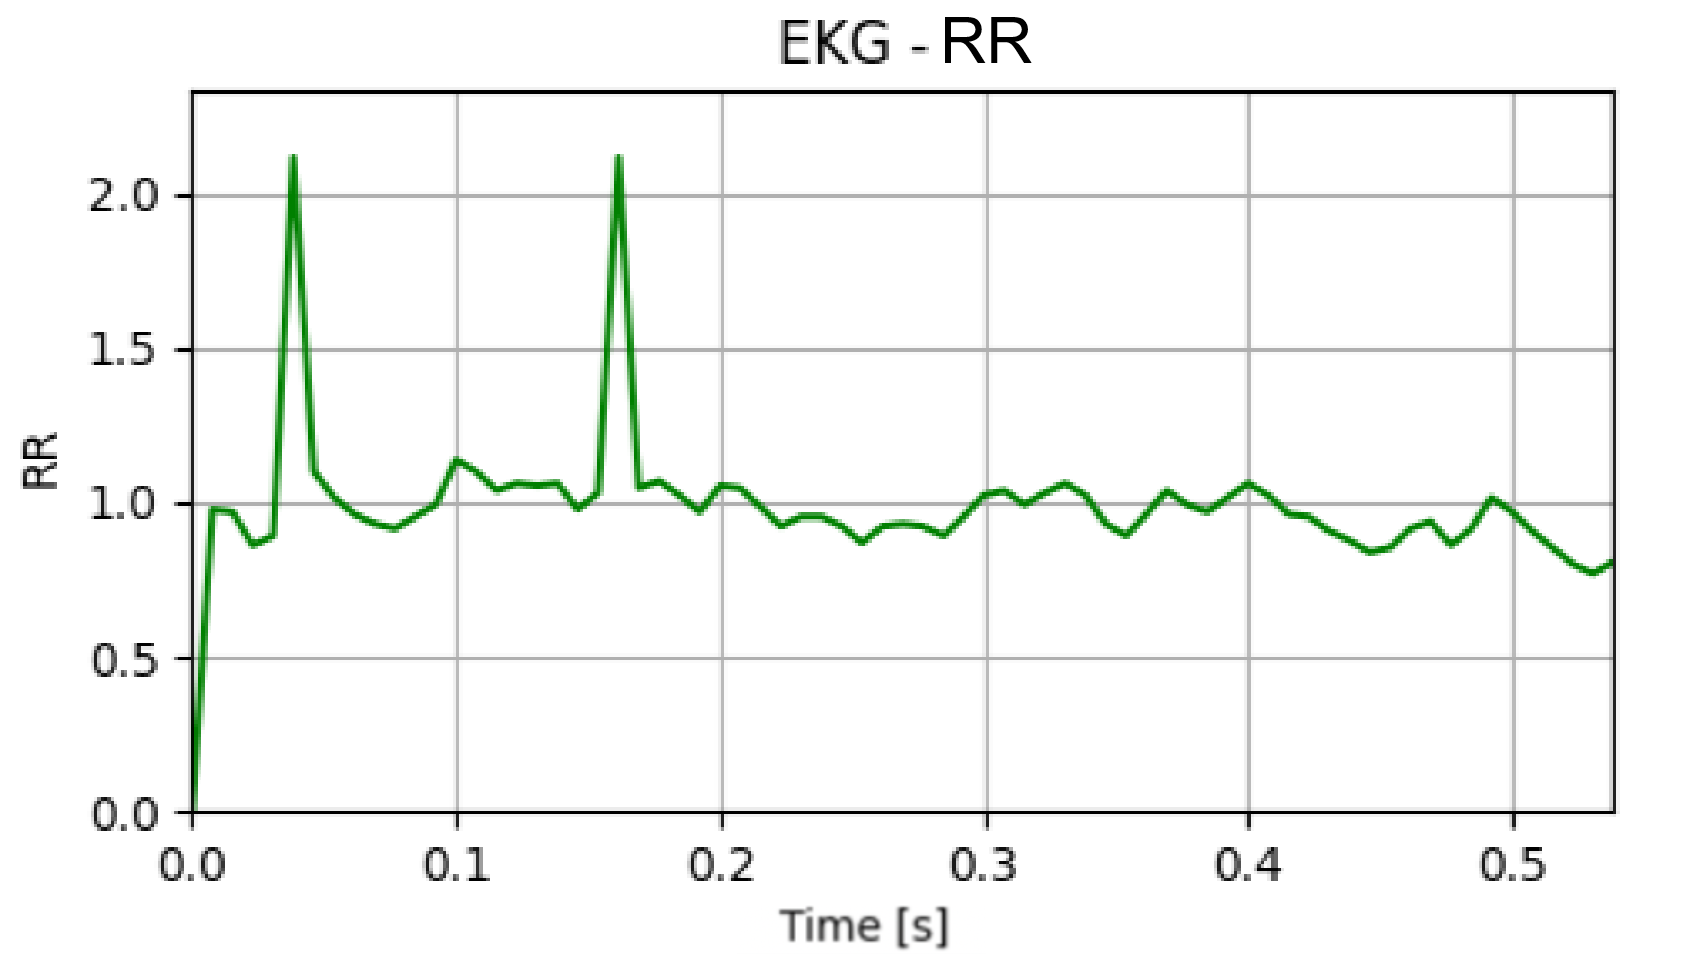
\includegraphics[width=\linewidth]{MEAN_EKG.png}
        \caption{RR intervals for ECG}
    \end{subfigure}
    
   \vspace{0.2cm} 
    \begin{subfigure}{0.49\textwidth}
        \centering
        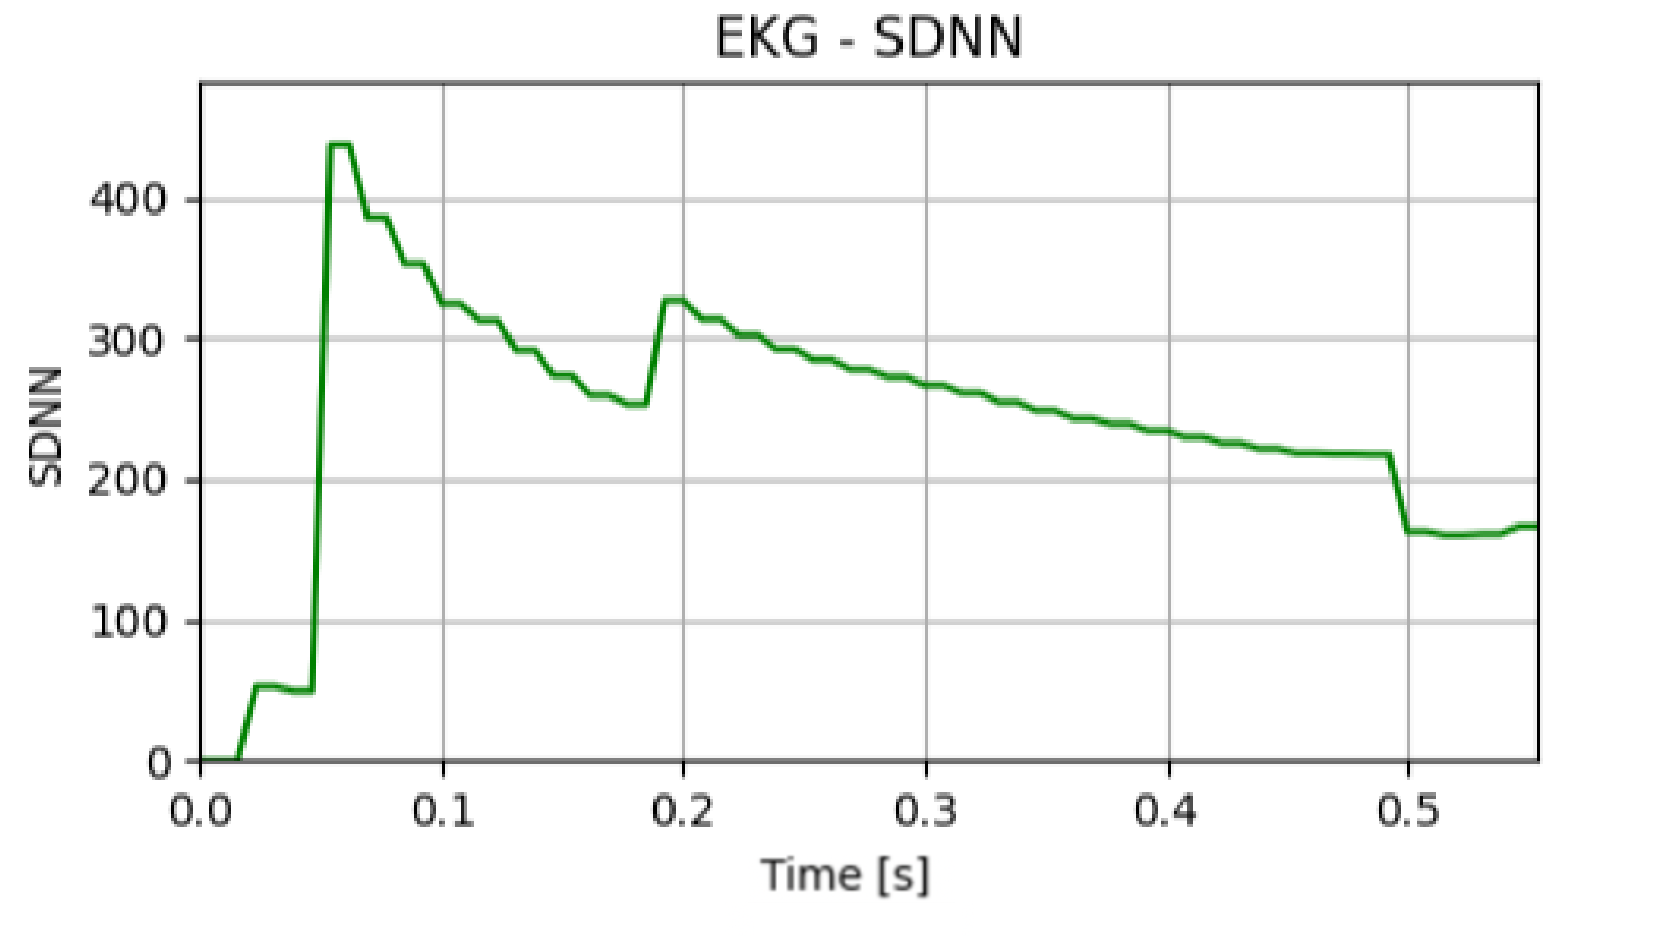
\includegraphics[width=\linewidth]{SDNN_EKG.png}
        \caption{Standard deviation of NN intervals}
    \end{subfigure}
    
    \vspace{0.2cm}  
    \begin{subfigure}{0.47\textwidth}
        \centering
        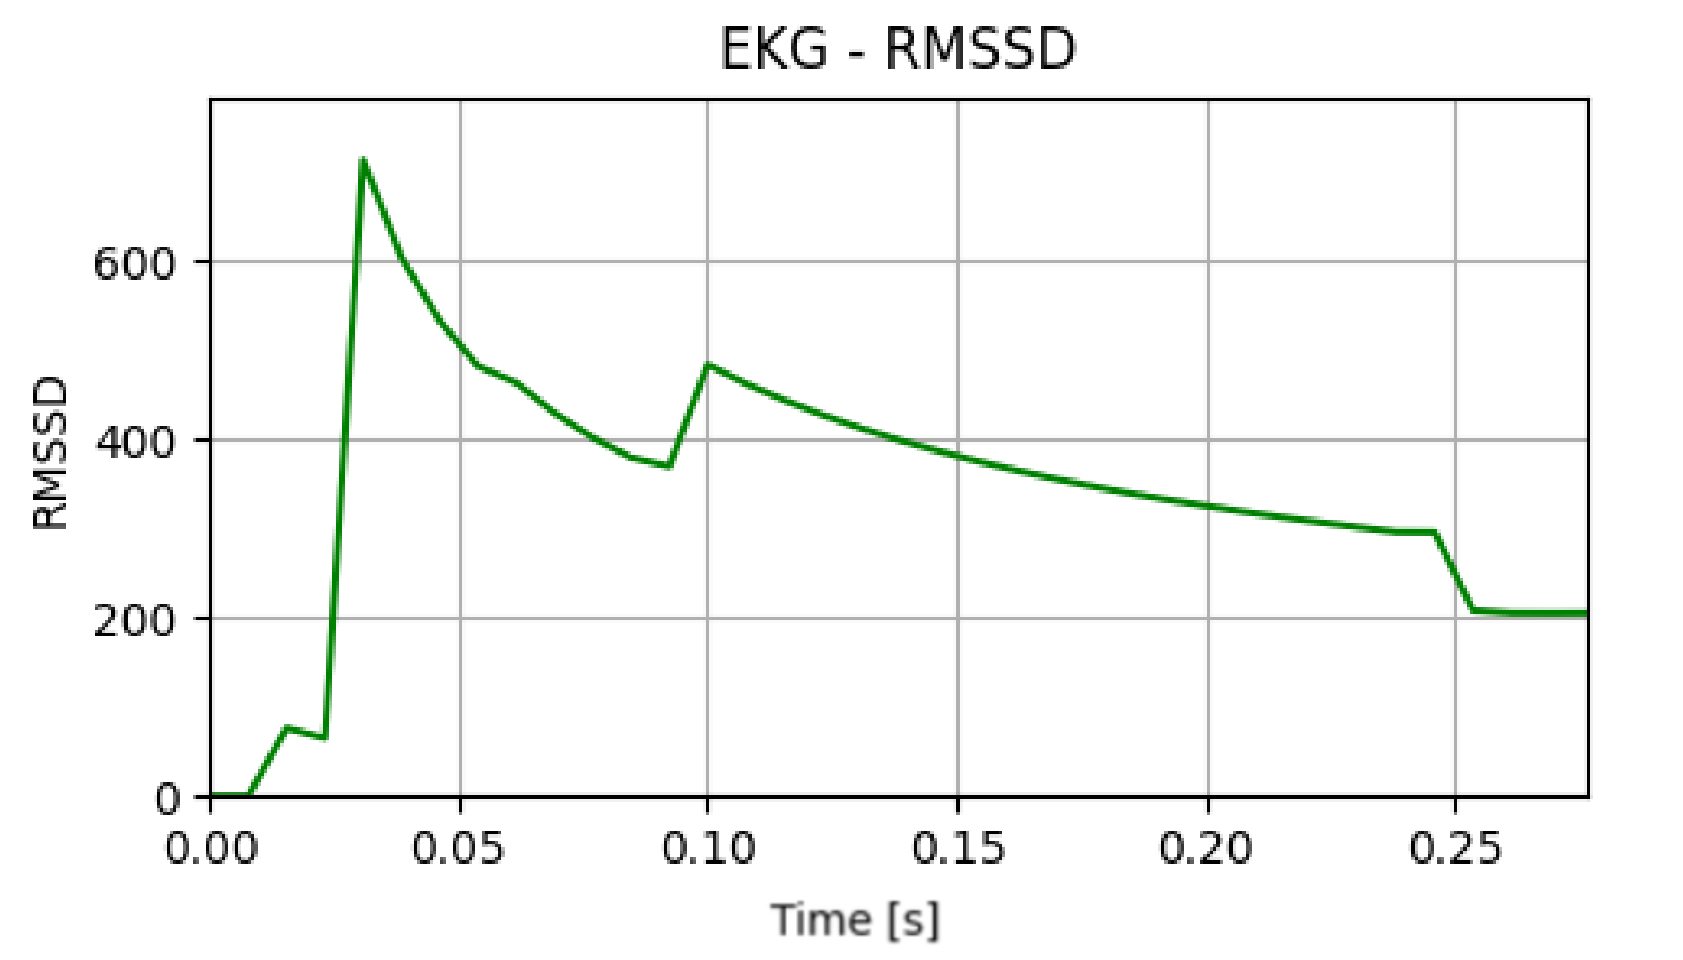
\includegraphics[width=\linewidth]{RMSSD_EKG.png}
        % NOTE:(mati): dumbest sentence ever
        \caption{Square root of an average of squares of differences of NN intervals}
    \end{subfigure}  
    \caption{Exemplary waveform of HRV indicators calculated for ECG}
\end{figure}

Comparison of HRV indicators between PPG and ECG methods showed that RMSSD and SDNN values calculated from ECG were more stable and less prone to sudden fluctuations. In the case of PPG, greater variability and occasional outlier values were observed. A possible explanation is the method’s susceptibility to interferences, such as variations in finger pressure against the camera.
%Porównanie wzkaźników HRV dla metody PPG i EKG wykazało, że wartości RMSSD i SDNN wyznaczone z EKG charakteryzują się większą stabilnością i mniejszą podatnością na skoki wartości. W przypadku PPG zauważalne były większe wahania oraz obecność pojedynczych wartości odstających, co wynika z podatności tej metody na zakłócenia, takie jak ruch czy zmienny nacisk palca na kamerę smartfona.

Despite the greater variability in PPG waveforms, the average HRV indicator values (SDNN and RMSSD) are similar to those obtained from ECG. This finding confirms that, under proper recording conditions, PPG can serve as a reliable alternative to ECG for heart rate variability analysis, although it requires additional filtering and artifact compensation.
%Pomimo większej zmienności w przebiegach PPG, średnie wartości wskaźników (SDNN i RMSSD) były zbliżone do uzyskanych dla EKG. Potwierdza to, że przy odpowiednich warunkach rejestracji PPG może stanowić wiarygodną alternatywę dla EKG w analizie zmienności rytmu serca, choć jego zastosowanie wymaga dodatkowych metod filtracji i kompensacji artefaktów.


\section{Summary}
Evaluation has shown that convolutional and recurrent architectures provide a high level of agreement with classical methods and reference data while minimizing false detections. The proposed models achieved high precision in detecting key points in the signals, with the F1 score reaching 0.9753 for R peaks in ECG signals and 0.9774 for wave peaks in PPG waveforms. The high accuracy of peak detection in photoplethysmographic signals demonstrates the strong potential of this method for reliably estimating IBIs, which are the counterparts of RR intervals in ECG signals.
% Ewaluacja wykazała, że zastosowane architektury splotowe i rekurencyjne zapewniają wysoką zgodność z klasycznymi metodami oraz danymi wzorcowymi, przy jednoczesnym ograniczeniu liczby fałszywych detekcji. %Uzyskane wartości miary F1 potwierdzają skuteczność analizy parametrów sercowo-naczyniowych  w warunkach mobilnych, niezależnie od poziomu aktywności fizycznej.
% fix number2:
%Zaproponowane metody osiągnęły wysoką skuteczność detekcji charakterystycznych punktów sygnału, uzyskując miarę F1 w detekcji załamków R równą 0,9753 dla elektrokardiografii, natomiast dla sygnału fotopletyzmograficznego przy wykrywaniu lokalnych szczytów uzyskano F1 równą 0,9774. %added2
%Średni interwał RR wyznaczony z EKG oraz interwał międzyuderzeniowy IBI z PPG różniły się średnio o około 5 ms. Różnica ta mieści się w granicach błędu pomiarowego i wskazuje na dużą zgodność między sygnałem pozyskiwanym za pomocą czujnika EKG a akwizycją PPG realizowaną smartfonem. %added3
%Wartości podstawowych parametrów HRV (SDNN, RMSSD) obliczone z PPG były bardzo zbliżone do tych z EKG, różnice mieściły się w granicach błędu pomiarowego.
%Zaproponowane modele osiągnęły wysoką precyzję w detekcji kluczowych punktów sygnału, uzyskując miarę F1 na poziomie 0,9753 dla załamków R w sygnale EKG oraz 0,9774 dla szczytów fali w przebiegu PPG.
%Wysoka dokładność detekcji pików w sygnale fotopletyzmograficznym świadczy o dużym potencjale tej metody do wiarygodnego szacowania interwałów międzyuderzeniowych IBI, które są odpowiednikiem interwałów RR z EKG.

Biomedical signal recording systems powered by machine learning methods show high potential for real-time health monitoring. Future efforts should focus on increasing the robustness of algorithms against environmental interferences, including motion artifacts, noise, and varying physiological conditions. It is also essential to develop mechanisms that enable integration with advanced telemedicine systems for continuous data uploading and analysis. Implementing these solutions could facilitate early identification of cardiac disorders and support clinical decision-making.
%Systemy rejestracji sygnałów biomedycznych, wspierane metodami uczenia maszynowego, wykazują potencjał w monitorowaniu stanu zdrowia w czasie rzeczywistym. Kolejne etapy prac powinny koncentrować się na zwiększenie odporności algorytmów detekcji na zakłócenia środowiskowe, w tym artefakty ruchowe, szumy oraz zmienne warunki fizjologiczne. Równocześnie kluczowe jest opracowanie mechanizmów integracji z zaawansowanymi systemami telemedycznymi, umożliwiającymi przesyłanie oraz analizę danych w sposób ciągły. Zastosowanie tych rozwiązań może wspierać wczesną identyfikację zaburzeń rytmu serca oraz wspomagać proces podejmowania decyzji klinicznych.

It is worth noting, however, that although the models have been trained on data that included interferences like sudden bodily movements or small finger shifting their validation happened in a controlled environment. From that an important limitation arises - there exists an uncertainty about system's behavior in real conditions, especially during intensive physical activity where movement becomes a dominating source of interferences. This problem is particularly clear in the PPG signal where instable contact of the detector with the skin may lead to significant measurement errors. There may exist improvements which would reduce the impact of the interferences on the results such as: applying adaptation filters which would dynamically correct their effect to account for the noise characteristic in the signal or usage of more complex deep learning models to process a variety of data.
%Warto jednak podkreślić, że choć modele trenowano na danych uwzględniających zakłócenia, takie jak nagłe ruchy ciała czy drobne poruszenia palca, ich walidacja odbyła się w warunkach kontrolowanych. Kluczowym ograniczeniem jest zatem niepewność co do zachowania systemu w warunkach rzeczywistych, zwłaszcza podczas intensywnej aktywności fizycznej, gdzie ruch staje się dominującym źródłem zniekształceń. Problem ten jest szczególnie widoczny w sygnale PPG, gdzie niestabilny kontakt czujnika ze skórą może prowadzić do znacznych błędów pomiarowych. Możliwe usprawnienia, które pozwolą zniwelować wpływ zakłóceń na rezultaty badań to: zastosowanie filtrów adaptacyjnych, które dynamicznie dostosowują swoje działanie do charakterystyki szumu w sygnale, lub wykorzystanie bardziej złożonych modeli uczenia głębokiego do przetwarzania zróżnicowanych danych.

\newpage

The developed system, including the source code, has been made publicly available on GitHub at the following repositories:
%Opracowany system wraz z kodem źródłowym został udostępniony publicznie w repozytoriach na GitHub pod adresami:

\noindent
\href{https://github.com/JanBancerewicz/PPGbetter}{https://github.com/JanBancerewicz/PPGbetter}
\href{https://github.com/JanBancerewicz/research-project}{https://github.com/JanBancerewicz/research-project}.

 

\begin{thebibliography}{1}
\bibitem{1}
C. Bronzino, J. D. Bronzino, “The Biomedical Engineering Handbook: Biomedical Signal Analysis”
\bibitem{2}
R. R. Sharma, R. B. Pachori, “Baseline Wander and Power Line Interference Removal from ECG Signals”, 2018
\bibitem{3}
S. Sörnmo, L. Laguna, “Bioelectrical Signal Processing in Cardiac and Neurological Applications”, 2005
\bibitem{4}
P. Podder, M. M. Hasan, M. R. Islam, M. Sayeed, “Design and Implementation of Butterworth, Chebyshev-I and Elliptic Filter for Speech Signal Analysis”, 2020
\bibitem{5}
M. R. Keshtkaran, Z. Yang, “A fast, robust algorithm for power line interference cancellation in neural recording”, 2014
\bibitem{6}
S. K. Mitra, “Digital Signal Processing: A Computer-Based Approach”
\bibitem{7}
Y. Yue, “An effective electrocardiogram segments denoising method based on EEMD, EMD, and wavelet packet”, IET Signal Processing
\bibitem{8}
S. Haykin, “Adaptive Filter Theory”, 5th ed., Pearson, 2013
\bibitem{9}
A. Hyvärinen, E. Oja, “Independent component analysis: algorithms and applications”
\bibitem{10}
O. Faust, U. R. Acharya, H. Adeli, A. Adeli, “Deep learning for healthcare applications based on physiological signals: A review”
\bibitem{11}
A. Boulif et al., “A literature review: ECG-based models for arrhythmia detection using AI techniques”, 2023
\bibitem{12}
Z. Ebrahimi, “A review on deep learning methods for ECG arrhythmia detection”
\bibitem{13}
D. A. Coast, R. M. Stern, G. G. Cano, S. A. Briller, “An approach to cardiac arrhythmia analysis using hidden Markov models”
\bibitem{14}
K. Kazemi, “Robust PPG Peak Detection Using Dilated Convolutional Neural Networks”
\bibitem{15}
S. Ikram et al., “Transformer-based ECG classification for early detection of cardiac arrhythmias”
\bibitem{16}
C. V. Nguyen, C. D. Do, “Transfer learning in ECG diagnosis: Is it effective?”
\bibitem{17}
W. Wang, L. Najafizadeh, “Ultra-Short Term Heart Rate Variability Estimation Using PPG and End-to-End Deep Learning”, 2024
\bibitem{18}
J. Xu, Y. Zhang, W. Wang, M. Xie, D. Zhu, “A Comprehensive PPG-based Dataset for HR/HRV Studies”, 2025
\bibitem{19}
B. De Ridder et al., “Smartphone Apps Using Photoplethysmography for Heart Rate Measurement: Systematic Review”
\bibitem{20}
J. D. Mather et al., “Validity of Resting Heart Rate Derived from Contact-Based Smartphone PPG”, 2024
\bibitem{21} 
Polar Electro, “Polar H10 heart rate sensor,” 2025
\bibitem{22} 
W. M. Laghari, M. Baloch, M. Mengal, S. Shah, “Performance Analysis of Analog Butterworth Low Pass Filter as Compared to Chebyshev Type-I Filter, Chebyshev Type-II Filter and Elliptical Filter”
\bibitem{23} 
S. Chakraborty, K. K. Jha, A. Patra, “Design of IIR Digital Highpass Butterworth Filter using Analog to Digital Mapping Technique”
\bibitem{24} 
G. Lenis, N. Pilia, A. Loewe, W. H. W. Schulze, O. Dössel, “Comparison of Baseline Wander Removal Techniques considering the Preservation of ST Changes in the Ischemic ECG: A Simulation Study”
\bibitem{25} 
R. J. Martis, U. R. Acharya, H. Adeli, “Current methods in electrocardiogram characterization”
\bibitem{26} 
M. A. F. Pimentel et al., “Toward a robust estimation of heart rate from wrist-type PPG signals”, 2016
\bibitem{27} 
J. Pan and W. J. Tompkins, “A real-time QRS detection algorithm”
\end{thebibliography}
\end{document}


